% =====================================================================
% 15_3nf_physics.tex
% 第 15 章 三核子力（3NF）的物理与低能常数
% Wave 5 / Chapter 15 (subagent)
% =====================================================================

\chapter{三核子力（3NF）的物理与低能常数}
\label{ch:15_3nf_physics}

% =========================================
\section{物理动机：为什么我们必须把 3NF 放进求解器}
\label{sec:ch15-motivation}

\subsection{两核子力是不是已经够用了？}
\label{subsec:ch15-2nf-not-enough}

\cref{ch:01_lippmann_schwinger,ch:02_two_body_numerics,ch:08_potential_matrix}
全部把"核力"理解成两体相互作用 \(\Vij{ij}{}\)：把它从相移、Deuteron 束缚能、
散射截面拟合出来，再放回 \cref{ch:04_faddeev_ags} 的 Faddeev/AGS 方程里
\textbf{原则上} 应该可以预言任何包含三个核子的可观测量。事实上现代高精度
两核子势——\texttt{Idaho\_N3LO} \cite{IdahoN3LO}、\texttt{N2LOopt}
\cite{N2LOopt}、\texttt{nijmegen} \cite{NijmegenII}——都做得相当好：它们
重现 \texttt{NN} 相移到 \(\sim 350\) MeV、Deuteron 静态性质（\(E_d, Q_d, \eta\)）
到 1\textperthousand 量级、电磁形状因子定性正确。

但当我们把这些两核子力放进三体——氚核（\(^3{\rm H}\)、\(^3{\rm He}\)）束缚态、
\(nd / pd\) 弹性散射、Breakup 反应——\textbf{系统性偏差} 立刻出现：

\begin{itemize}
\item \textbf{氚核结合能不足}（"underbinding"）。实验值
      \(B(^3{\rm H}) = 8.482\) MeV，纯 2NF 计算给出 \(7.6\)–\(7.9\) MeV，
      偏少 \(0.5\)–\(0.9\) MeV，对应相对误差 \(\sim 7\%\)。这个差额在
      \(^3{\rm He}\) 与 \(^4{\rm He}\) 上更大。
\item \(\boldsymbol{Ay}\) \textbf{谜题（\(Ay\) puzzle）}。\(nd\) 弹性散射在
      \(\Tlab \sim 5\)–\(30\) MeV 的极化分析能力 \(Ay\) 在 \(\theta_{\rm cm} \sim 100^\circ\)
      处理论低于实验约 \(30\%\)。这一差额对实空间 \(NN\) 相移不敏感，
      却对 \(P\)-波 NN 张量耦合的 \emph{某种 3 体修正} 极为敏感——这正是
      "极化谜题"的核心。
\item \(\boldsymbol{nd}\) \textbf{微分截面在中等能量（\(\Tlab \gtrsim 100\) MeV）
      的极小值（minimum）漂移}。在 \(\theta_{\rm cm} \approx 120^\circ\)
      附近 \(d\sigma/d\Omega\) 的极小值实验上比纯 2NF 预言低 \(15\%\)–\(25\%\)，
      被认为是 3NF "重新分配" 自旋通道权重的间接信号。
\item \textbf{Breakup 截面的 SST/QFS 配置}。"对称空间星（Space-Star）"和
      "Quasi-Free Scattering（QFS）"两类极端 3 体几何，对 \(NN\) 几乎不敏感
      （主要由相空间决定），却在多个能量上系统性高于或低于 2NF 预言
      \(10\%\)–\(20\%\)。
\end{itemize}

这些不是"势模型选不对"的问题——所有现代 \texttt{NN} 势同时偏差且
偏差方向一致。它是一个\textbf{结构性遗漏}：三个核子\emph{不能}被简单地
表示为两两两体相互作用的总和。这就是\textbf{三核子力}（three-nucleon force,
3NF）登场的物理动机。

\subsection{Power counting 视角：3NF 是 \({\rm N}^2{\rm LO}\) 起步的常态}
\label{subsec:ch15-power-counting}

手征有效场论（chiral effective field theory, ChEFT）对核力的展开按照
\textbf{动量比例 \(Q/\Lambda_\chi\)} 的幂次组织（\(Q \sim m_\pi\)
是低动量标度；\(\Lambda_\chi \sim 1\) GeV 是手征对称破缺标度）。
Weinberg 的 \emph{naive dimensional analysis} 给出的 3NF 出现阶数：

\begin{table}[h]
\centering
\caption{ChEFT 中两体力（2NF）与三体力（3NF）按 Weinberg power counting 出现的阶。}
\label{tab:ch15-power-counting}
\begin{tabular}{l c c c}
\toprule
阶数 & 名称 & 2NF & 3NF \\
\midrule
\(\nu = 0\) & LO     & 含接触项 + 1\(\pi\) 交换 & ---（被 \(\delta\) 函数吸收，无新结构）\\
\(\nu = 2\) & NLO    & 2\(\pi\) 交换 + 接触项   & ---（cancellations，文献证明 \(=0\)）\\
\(\nu = 3\) & N\({}^2\)LO & N\(^2\)LO 修正 & \textbf{首次出现}（\(c_1, c_3, c_4, c_D, c_E\)）\\
\(\nu = 4\) & N\({}^3\)LO & N\(^3\)LO 修正 & 全 N\(^3\)LO 3NF（许多新拓扑）\\
\bottomrule
\end{tabular}
\end{table}

关键结论：\textbf{3NF 在 N\(^2\)LO 阶（与 2NF 的 N\(^2\)LO 修正同一阶）
首次出现，并且只引入 5 个新低能常数 \(\cone, \cthree, \cfour, \cD, \cE\)}。
其中 \(\cone, \cthree, \cfour\) 与 2NF 的 N\(^2\)LO 长程项共用同一个
\(\pi N\) 拉氏量项，因此它们的数值\textbf{从 2NF 拟合中已经定下}，
3NF 不需要重新拟合（这就是 Tic-tac 中
\texttt{three\_nucleon\_force\_model::fetch} 把 \(c_i\) 从 2NF 模型读
出的原因——见 \cref{lst:ch15-tnf-factory}）。剩下的 \(\cD, \cE\) 是
3NF \emph{独有的} 低能常数，需要用三体可观测量（如 \(B(^3{\rm H})\) 或
\(nd\) 双普林相对论截面）拟合。

这一 power counting 也解释了为什么 \(Ay\) 谜题"难解"——\(Ay\) 来自
NN 自旋三重态中的张量分量与 spectator 之间的 \emph{自旋} 耦合，需要的是
正确处理 \(\cthree, \cfour\)（两 \(\pi\) 交换中 spectator 与配对粒子之间的
张量结构），而 \(\cone\) 项的 spin-isospin 结构相对简单。

\subsection{\(nd\) 散射中的"敏感窗口"}
\label{subsec:ch15-sensitivity-windows}

不同 3NF 项对不同 \(nd\) 可观测量的敏感度不同。下表汇总文献
\cite{Epelbaum2002NLO3NF, Witala1988, Miller2023PRC} 中的"敏感窗口"
（sensitivity window），帮助理解为什么 Tic-tac 把整个 3NF 项乘以
\texttt{w1\_scale} 因子做扫描：

\begin{table}[h]
\centering
\caption{N\(^2\)LO 3NF 各项对 \(nd\) 弹性散射可观测量的敏感度（\(\bullet\) = 强敏感；
\(\circ\) = 弱敏感）。"\(\Tlab\) 区"是该敏感度最大的能量窗口。}
\label{tab:ch15-sensitivity}
\begin{tabular}{l c c c c c c}
\toprule
项 & LEC & \(\diffXS_{\min}\) & \(\Ay\) & \(\iTeleven\) & \(\Ttwentyzero\) & \(\Tlab\) 区 [MeV] \\
\midrule
2\(\pi\)-exchange (rank-0) & \(\cone\)        & \(\bullet\) & \(\circ\)   & \(\bullet\) & \(\bullet\) & 60--250 \\
2\(\pi\)-exchange (rank-2) & \(\cthree\)      & \(\bullet\) & \(\bullet\) & \(\bullet\) & \(\bullet\) & 100--250 \\
2\(\pi\)-exchange (\(\cfour\) tensor) & \(\cfour\)  & \(\circ\)   & \(\bullet\) & \(\circ\)   & \(\circ\)   & 5--30 \\
1\(\pi\)-CT & \(\cD\)        & \(\circ\)   & \(\bullet\) & \(\circ\)   & \(\circ\)   & 5--30 \\
3N-CT  & \(\cE\)        & \(\bullet\) & \(\circ\)   & \(\bullet\) & \(\circ\)   & 任意（与 \(\Tlab\) 关系弱） \\
\bottomrule
\end{tabular}
\end{table}

注意 \(\cfour\) 与 \(\cD\) 都是 \(Ay\) 谜题的关键候选；这正是为什么
低能（\(\Tlab \sim 10\) MeV）极化数据成为 ChEFT 3NF 拟合的"金标准"。
本书（Tic-tac）的 canonical benchmark \(\Tlab = 190\) MeV 落在 2\(\pi\)-exchange
强敏感的区段，因此可以用来验证 \(\cone, \cthree\) 项的实现。

\subsection{本章的目标}
\label{subsec:ch15-goals}

读完本章你应能：
\begin{itemize}
\item 在纸笔上独立写出 N\(^2\)LO 3NF 三大类项（2\(\pi\)-exchange、1\(\pi\)-CT、
      3N-CT）的算符形式与低能常数依赖；
\item 知道 \(\cone, \cthree, \cfour\) 为什么"从 2NF 继承"以及在哪个文件
      （\texttt{include/constants.h}）里被存为常数；
\item 理解 \(\cD, \cE\) 的定义、单位、文献符号约定的歧义（Epelbaum vs
      Navrátil vs Witała 三套），并知道 Tic-tac 选了哪一套（commit
      \texttt{f4df358} 修复后的 +½ 规范）；
\item 看到 \texttt{three\_nucleon\_force\_model.h} 的接口立刻知道
      \texttt{enabled()}, \texttt{W1\_element()} 各自对应数学上的什么；
\item 跑出一个开 / 关 3NF 的 \(\diffXS\) 对照，并在固定通道上读出 3NF/2NF 强度比；
\item 知道与 \cref{ch:08_potential_matrix} 的两体 \(V\) 矩阵、与
      \cref{ch:11_faddeev_solver} 的求解器、以及与 \cref{ch:16_3nf_pw_projection}
      的部分波投影代码三处接口分别长什么样。
\end{itemize}

\cref{ch:16_3nf_pw_projection,ch:17_3nf_numerical} 会承接本章，详细展开
部分波重耦合系数的代数推导（rank-0 / rank-2 / 9j / CG）以及实际数值代码
的内层热路径。本章把"\textbf{物理 + LEC + 接口}"讲透，留给下两章
"\textbf{代数细节 + 内循环代码}"。

% =========================================
\section{数学推导：N\({}^2\)LO 3NF 的三个组分}
\label{sec:ch15-math}

整章最长的一节。我们逐项推导 N\(^2\)LO 3NF 的算符形式。基础
拉氏量取手征对称的形式，包含核子场 \(N\)、\(\pi\) 介子场 \(\pi\) 与
"低能常数"\(\cone, \cthree, \cfour, \cD, \cE\)。所有动量都用 fm\(^{-1}\)
（用 \(\hbarc = 197.327\) MeV·fm 转换）。

\subsection{基础拉氏量与三个 vertex 拓扑}
\label{subsec:ch15-lagrangian}

ChEFT 重子部分的有效拉氏量按手征展开 \cite{Epelbaum2002NLO3NF}：

\begin{equation}
\label{eq:ch15-Leff}
\mathcal{L}_{\rm eff}
= \mathcal{L}^{(0)}_{\pi N} + \mathcal{L}^{(1)}_{\pi N} + \mathcal{L}^{(2)}_{\pi N}
+ \mathcal{L}^{(0)}_{NN} + \mathcal{L}^{(2)}_{NN}
+ \mathcal{L}^{(1)}_{\pi NN} + \mathcal{L}^{(0)}_{NNN} + \cdots
\end{equation}

按 power counting，N\(^2\)LO 3NF 涉及的拉氏量项是：

\begin{align}
\label{eq:ch15-LpiN-c-terms}
\mathcal{L}^{(2)}_{\pi N}
&\supset
\bar{N} \Big[ 2 \cone \, m_\pi^2 \,(\pi^2/\fpi^2)
       - \tfrac{\cthree}{\fpi^2}\, (\partial_\mu \pi)^a (\partial^\mu \pi)^a
       + \tfrac{\cfour}{2\fpi^2}\, \epsilon^{abc} \tau^c
            \sigma^{\mu\nu} (\partial_\mu \pi)^a (\partial_\nu \pi)^b
       \Big] N \\
\label{eq:ch15-LpiNN-cD}
\mathcal{L}^{(1)}_{\pi NN}
&\supset
- \frac{\cD}{\fpi^2 \Lambda_\chi}\,
   \big( \bar{N} \tau^a \bvec{\sigma} N \big)
   \cdot \big( \bar{N} N \big)\,
   \partial^a \pi^a \\
\label{eq:ch15-LNNN-cE}
\mathcal{L}^{(0)}_{NNN}
&\supset
- \frac{\cE}{2 \fpi^4 \Lambda_\chi}\,
   \big( \bar{N} N \big)\, \big( \bar{N} \bvec{\tau} N \big)
   \cdot \big( \bar{N} \bvec{\tau} N \big)
\end{align}

注意三个量纲：
\begin{itemize}
\item \(\cone, \cthree, \cfour\) 量纲 \([\rm GeV]^{-1}\)（Tic-tac 内部转成 fm，
      因子 \(\hbarc/1000 \approx 0.197\)）。物理意义：\textbf{\(\pi N\) sigma
      term 的低能展开}，从 \(\pi N\) 散射拟合。
\item \(\cD\) \emph{无量纲}。物理意义：\textbf{NN-\(\pi\)-NN 接触顶点}。
      与 2NF 的同名 \(\cD\) \emph{共享}（这是 Epelbaum 引入它的目的——
      让 1\(\pi\) exchange 与短程接触在同一拓扑下重新组合，避免双计入）。
\item \(\cE\) \emph{无量纲}。物理意义：\textbf{纯 3 核子接触顶点}。
      量纲补偿因子 \(\fpi^4 \Lambda_\chi\) 让 \(\cE\) 自然成 \(O(1)\)。
\end{itemize}

把这些拉氏量项的 vertex 与传播子组合，给出 N\(^2\)LO 3NF 的三个 Feynman 拓扑：

\begin{figure}[h]
\centering
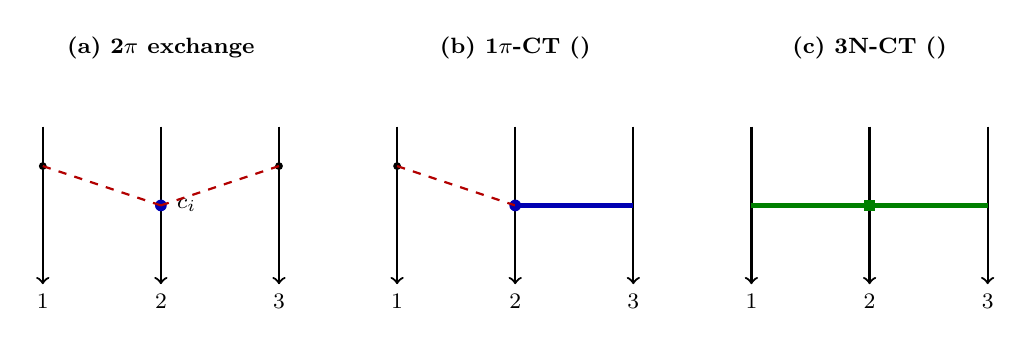
\begin{tikzpicture}[
  node distance=4mm and 8mm,
  every node/.style={font=\footnotesize, align=center},
  nucl/.style={->, thick},
  pi/.style={dashed, thick, draw=red!70!black},
  vert/.style={circle, fill=black, inner sep=1pt},
  cvert/.style={circle, fill=blue!70!black, inner sep=1.5pt},
  evert/.style={rectangle, fill=green!50!black, inner sep=2pt}
]
  % --- (a) 2pi-exchange ---
  \node at (-1.5,3) {\textbf{(a) 2\(\pi\) exchange}};
  \draw[nucl] (-3,2) -- (-3,0);
  \draw[nucl] (-1.5,2) -- (-1.5,0);
  \draw[nucl] ( 0,2) -- ( 0,0);
  \node[vert] at (-3,1.5) {};
  \node[cvert, label=right:{\(c_i\)}] at (-1.5,1.0) {};
  \node[vert] at ( 0,1.5) {};
  \draw[pi] (-3,1.5) -- (-1.5,1.0);
  \draw[pi] ( 0,1.5) -- (-1.5,1.0);
  \node[below] at (-3,0) {1};
  \node[below] at (-1.5,0) {2};
  \node[below] at ( 0,0) {3};

  % --- (b) 1pi-CT ---
  \node at (3.0,3) {\textbf{(b) 1\(\pi\)-CT (\(\cD\))}};
  \draw[nucl] ( 1.5,2) -- ( 1.5,0);
  \draw[nucl] ( 3.0,2) -- ( 3.0,0);
  \draw[nucl] ( 4.5,2) -- ( 4.5,0);
  \node[vert] at ( 1.5,1.5) {};
  \node[cvert, label=right:{\(\cD\)}] at ( 3.0,1.0) {};
  \draw[pi] ( 1.5,1.5) -- ( 3.0,1.0);
  \draw[ultra thick, draw=blue!70!black] ( 3.0,1.0) -- ( 4.5,1.0);
  \node[below] at ( 1.5,0) {1};
  \node[below] at ( 3.0,0) {2};
  \node[below] at ( 4.5,0) {3};

  % --- (c) 3N-CT ---
  \node at (7.5,3) {\textbf{(c) 3N-CT (\(\cE\))}};
  \draw[nucl] ( 6.0,2) -- ( 6.0,0);
  \draw[nucl] ( 7.5,2) -- ( 7.5,0);
  \draw[nucl] ( 9.0,2) -- ( 9.0,0);
  \node[evert, label=right:{\(\cE\)}] at ( 7.5,1.0) {};
  \draw[ultra thick, draw=green!50!black] ( 6.0,1.0) -- ( 7.5,1.0);
  \draw[ultra thick, draw=green!50!black] ( 7.5,1.0) -- ( 9.0,1.0);
  \node[below] at ( 6.0,0) {1};
  \node[below] at ( 7.5,0) {2};
  \node[below] at ( 9.0,0) {3};
\end{tikzpicture}
\caption{N\(^2\)LO 3NF 的三个 Feynman 拓扑。
(a) 双 \(\pi\) 交换：粒子 1 与 3 各自交换一个 \(\pi\) 介子，
中央顶点（蓝点）是 \(\pi N\) 的 \(c_1 / c_3 / c_4\) 接触项。
(b) 1\(\pi\)-CT：粒子 1 与 2 之间交换一个 \(\pi\)；
粒子 2 与 3 之间是 \(\cD\) 接触（蓝色厚线）。
(c) 纯 3N 接触：三粒子线在同一点（\(\cE\) 顶点，绿方块）相遇。}
\label{fig:ch15-topologies}
\end{figure}

\textbf{物理类比：每条线段对应什么。} \(\pi\) 交换线段（红虚线）的传播子是
\(1/(q^2 + m_\pi^2)\)；它把"动量 \(q\)"从一个核子传到另一个；动量越大、
\(\pi\) 介子离 mass shell 越远、传播子越小，\textbf{这就是为什么 3NF 的
"作用半径"约 \(1/m_\pi \approx 1.4\) fm}。蓝厚线代表"接触项"
（contact term，无传播子，直接由低能常数 \(\cD\) 描述瞬时短程相互作用）。
绿方块同理表示纯 3 体接触。

\subsection{spectator-1 分解与 \(W^{(1)}\)}
\label{subsec:ch15-spectator-1}

3NF 的全算符可以按"哪个粒子是 spectator"自然分成三段：
\begin{equation}
\label{eq:ch15-3NF-decomp}
W = W^{(1)} + W^{(2)} + W^{(3)},
\qquad
W^{(i)} \equiv \text{(spectator-\(i\) 分量)}.
\end{equation}

\(W^{(1)}\) 是"粒子 1 不动、粒子 2 与 3 之间作用"的部分。利用全同粒子
循环对称性
\begin{equation}
\label{eq:ch15-W-cyclic}
W^{(2)} = \Pop_{123}\, W^{(1)}\, \Pop_{123}^{-1},
\quad
W^{(3)} = \Pop_{132}\, W^{(1)}\, \Pop_{132}^{-1},
\end{equation}
（其中 \(\Pop_{123}, \Pop_{132}\) 是 \cref{ch:09_permutation_p123} 的循环置换），
全 3NF 算符可以由\textbf{单一}的 \(W^{(1)}\) 完全恢复：
\begin{equation}
\label{eq:ch15-W-full}
W = (1 + \Pop_{123} + \Pop_{132})\, W^{(1)} = (1 + \Pop)\, W^{(1)},
\end{equation}
\(\Pop = \Pop_{123} + \Pop_{132}\) 即 \cref{eq:ch04-P-sum-def} 的同一对象。
这一 trick 把"实现 3NF"压缩为"实现 \(W^{(1)}\)"——只要把 spectator-1
矩阵元算对、外层求解器自然把 \(W^{(2,3)}\) 通过 \(\Pop\) 帮你算了。
代码 \texttt{three\_nucleon\_force\_model::W1\_element} 接口正是这一
分解的直接对应（\cref{lst:ch15-tnf-abstract}）。

\subsection{2\(\pi\)-exchange 项 \(W^{(1)}_{2\pi}\)（Fujita-Miyazawa 类）}
\label{subsec:ch15-2pe}

历史上 \cite{Epelbaum2002NLO3NF} 第一个被引入的 3NF 形式是 1957 年
Fujita 与 Miyazawa 给出的，后被 Epelbaum 等人整合到 ChEFT 框架。
其 spectator-1 算符为
\begin{equation}
\label{eq:ch15-W2pe-op}
\boxed{
W^{(1)}_{2\pi} = \left( \frac{g_A}{2 \fpi} \right)^{\!2}\,
\frac{(\bvec{\sigma}_2 \cdot \bvec{q}_2)\,(\bvec{\sigma}_3 \cdot \bvec{q}_3)}
     {(q_2^2 + m_\pi^2)(q_3^2 + m_\pi^2)}\,
(\bvec{\tau}_2 \cdot \bvec{\tau}_3)\,
F_{c_1 c_3}(q_2, q_3)
}
\end{equation}
其中
\begin{equation}
\label{eq:ch15-F-c1c3}
F_{c_1 c_3}(q_2, q_3) = -\frac{4 \cone\, m_\pi^2}{\fpi^2} + \frac{2\, \cthree\,
(\bvec{q}_2 \cdot \bvec{q}_3)}{\fpi^2},
\end{equation}
而 \(\bvec{q}_2 = \bvec{p} - \bvec{p}' + \tfrac{1}{2}(\bvec{q}' - \bvec{q})\)
与 \(\bvec{q}_3 = -\bvec{p} + \bvec{p}' + \tfrac{1}{2}(\bvec{q}' - \bvec{q})\)
是粒子 2 / 3 各自吸收的 \(\pi\) 介子动量（在 spectator-1 Jacobi 坐标下）。
\(\cfour\) 项含 \(\bvec{\tau}_1 \cdot (\bvec{\tau}_2 \times \bvec{\tau}_3)\)
的同位旋叉积，需要 spectator 与 pair 之间的同位旋耦合，结构最复杂；
当前 Tic-tac 实现\textbf{暂未开启 \(\cfour\)}（详见 \cref{lst:ch15-N2LO-3NF-class}
中 \texttt{m\_c4} 字段被声明但 \texttt{W1\_element} 不调用它）。

\paragraph{各 LEC 的物理意义。}
\begin{description}
\item[\(\cone\)：\(\pi N\) sigma term + scalar isoscalar 介子尾部。]
\(\cone \sim -1\) \(\rm GeV^{-1}\)（实验拟合值约 \(-0.81\)–\(-0.92\)
\(\rm GeV^{-1}\)）。它的物理来源是 \(\pi N\) 散射的 \emph{Born 散射长度}；
在 dispersion 表象里，\(\cone\) 吸收了 \(\sigma\) 介子（\(\sim 500\)–\(600\) MeV
的 \(\pi\pi\) 共振）的尾部贡献。从 \(\pi N\) 散射 sub-threshold 数据
拟合得 \(\cone^{\rm phen} = -0.81 \pm 0.15\) \(\rm GeV^{-1}\)
\cite{Epelbaum2002NLO3NF}。
\item[\(\cthree\)：scalar mesons + \(\Delta\) isobar 通道。]
\(\cthree \sim -3.4\) \(\rm GeV^{-1}\)，绝对值最大、对 3NF 数值贡献\textbf{最强}。
物理来源：\(\Delta(1232)\) isobar 中间态的"积分掉"贡献（\(\Delta\) 隐式
出现）+ scalar 介子尾部。直接看：在 \(\Delta\)-full ChEFT 里
\(\cthree = \cthree^{\rm w/o\,\Delta} + \cthree^{\Delta}\)，其中
\(\cthree^{\Delta} \approx -2 g_A^2/(9 \Delta_M)\) （\(\Delta_M = M_\Delta - M_N
\approx 293\) MeV）给出绝大部分（\(\sim -2.7\) \(\rm GeV^{-1}\)）。
这就是为什么\textbf{包含 \(\Delta\) 的 ChEFT 与 \(\Delta\)-less ChEFT
拟合 \(\cthree\) 时数值差异巨大}——一个 \(\sim -1\)，另一个 \(\sim -3\)。
\item[\(\cfour\)：vector mesons + \(\Delta\) isobar 通道。]
\(\cfour \sim +4\) \(\rm GeV^{-1}\)，符号与 \(\cthree\) 相反、绝对值近似相等。
物理来源：\(\rho\) 介子（\(\sim 770\) MeV）尾部 + \(\Delta\) 通道。\(\cfour\)
项的 spin-isospin 结构（\(\bvec{\tau}_1 \cdot (\bvec{\tau}_2 \times \bvec{\tau}_3)\)
\(\bvec{\sigma}_1 \cdot (\bvec{\sigma}_2 \times \bvec{\sigma}_3) \cdot \cdots\)）
是 \(Ay\) 谜题的关键怀疑对象——它对低能极化非常敏感
但对相移和无极化截面贡献小。
\end{description}

\paragraph{rank-0 + rank-2 分解。}
算符 \((\bvec{\sigma}_2 \cdot \bvec{q}_2)(\bvec{\sigma}_3 \cdot \bvec{q}_3)\)
是 \(\bvec{\sigma}_2\) 与 \(\bvec{\sigma}_3\) 的张量积、缩并到两个动量。
按球张量代数（\cref{ch:03_jacobi_partial_wave}）的 rank 分解：
\begin{equation}
\label{eq:ch15-rank0-rank2-2pe}
(\bvec{\sigma}_2 \cdot \bvec{q}_2)(\bvec{\sigma}_3 \cdot \bvec{q}_3)
= \tfrac{1}{3}\,(\bvec{\sigma}_2 \cdot \bvec{\sigma}_3)\,(\bvec{q}_2 \cdot \bvec{q}_3)
+ [\bvec{\sigma}_2 \otimes \bvec{\sigma}_3]_2 \cdot [\bvec{q}_2 \otimes \bvec{q}_3]_2,
\end{equation}
即 \emph{rank-0（标量）} 与 \emph{rank-2（张量）} 之和。rank-0 在部分波
基底里只允许 \(L_{2N} = L_{2N}'\)（pair 轨道角动量不变），rank-2 则
\textbf{允许 \(L_{2N} \to L_{2N} \pm 2\)}（最经典的就是 \({}^3S_1 \leftrightarrow {}^3D_1\)
耦合）。这是为什么 Tic-tac 的实现里 \texttt{W1\_2pe} 必须对 \emph{两个}
recoupling helper（\texttt{recoupling\_3nf\_scalar} 与
\texttt{recoupling\_3nf\_rank2}）分别调用——前者实现 rank-0、后者实现 rank-2，
rank-2 是 \(Ay\) 改善的"分子"项。
\cref{ch:16_3nf_pw_projection} 会逐步推导这两个 helper 的代数细节。

\subsection{1\(\pi\)-CT 项 \(W^{(1)}_{1\pi-{\rm CT}}\)（\(\cD\)）}
\label{subsec:ch15-1pe-ct}

spectator-1 与 pair 之间的"1\(\pi\) 交换 + 配对接触"结构。
spectator-1 算符：
\begin{equation}
\label{eq:ch15-W1pe-ct-op}
\boxed{
W^{(1)}_{1\pi-{\rm CT}}
= -\frac{g_A\, \cD}{8\, \fpi^4\, \Lambda_\chi} \times 2 \times
\sum_{j=2,3}\,
\frac{(\bvec{\tau}_1 \cdot \bvec{\tau}_j)\,(\bvec{\sigma}_1 \cdot \hat{q}_j)\,(\bvec{\sigma}_j \cdot \hat{q}_j)}
     {q_j^2 + m_\pi^2}
}
\end{equation}
（求和的"\(\times 2\)"在 Tic-tac 实现里被显式吸进总系数；见
\texttt{chiral\_N2LO\_3NF.h:248}）。物理图：\(\pi\) 介子从 spectator 1
出发、传到 pair 中的某一粒子（\(j\)），同时 pair 内的另一粒子通过 \(\cD\)
接触顶点直接相互作用。

\paragraph{为什么 1\(\pi\)-CT 与 NN 的 \(\cD\) 共享。}
拉氏量 \cref{eq:ch15-LpiNN-cD} 同时给出"两体内部" 与 "三体" 两个图
（在两体里它是"\(\pi\) 散射 + 接触" 修正，在三体里是上述 1\(\pi\)-CT
拓扑）。\textbf{两个图的 \(\cD\) 必须相同}，否则 ChEFT 会有低能常数
"双重定义"——这是 Epelbaum 把 \(\cD\) 这个名字从 NN 顶点借到 3NF 的
原因。Tic-tac 的 \texttt{c\_D} 参数读自输入文件，\textbf{用户负责保证它
和 NN 部分的 \(\cD\) 数值一致}（默认输入用 Witała 给出的 \(\cD = -0.2\)
\cite{Epelbaum2002NLO3NF}）。

\paragraph{选择规则。}
1\(\pi\)-CT 的 pair vertex 是接触项（不带任何动量 / 角动量），所以它
\emph{只允许} pair 的 \emph{S 波}（\(L_{2N} = 0\)）。这一选择规则在代码里
由 \texttt{recoupling\_3nf\_1pe\_ct\_scalar} 的内部
\texttt{if (L\_2N\_r != 0 || L\_2N\_c != 0) return 0.0} 短路实现。
同时 spectator 的轨道，因此 \(L_{1N} = L_{1N}'\)。

\paragraph{rank-0 + rank-2 分解。}
\((\bvec{\sigma}_1 \cdot \hat{q})(\bvec{\sigma}_3 \cdot \hat{q})\) 与 2PE 的
\((\bvec{\sigma}_2 \cdot \bvec{q}_2)(\bvec{\sigma}_3 \cdot \bvec{q}_3)\)
形式上同构，只是这里两个 \(\hat{q}\) 是\textbf{同一个}单位矢量（即
spectator 动量传 \(\Delta \bvec{q} = \bvec{q}' - \bvec{q}\) 的方向）。
所以分解为
\begin{equation}
\label{eq:ch15-rank0-rank2-1pe}
(\bvec{\sigma}_1 \cdot \hat{q})(\bvec{\sigma}_3 \cdot \hat{q})
= \tfrac{1}{3}\,(\bvec{\sigma}_1 \cdot \bvec{\sigma}_3)
+ [\bvec{\sigma}_1 \otimes \bvec{\sigma}_3]_2 \cdot [\hat{q} \otimes \hat{q}]_2.
\end{equation}
注意 rank-2 的空间部分是 \emph{Y\(_2(\hat{q})\)}，作用在 \emph{spectator 方向}
（不是 pair 方向）。在部分波展开里它要求 \(L_{1N} \to L_{1N} \pm 2\)；
对 \(L_{1N} = L_{1N}' = 0\)（即 spectator 是 S 波，氚核主分量）由 CG
选择规则
\begin{equation}
\langle 0\, 0 | 2\, 0 | 0\, 0 \rangle = 0
\end{equation}
\textbf{自动消失}。所以 1\(\pi\)-CT 的 rank-2 项只在更高 \(L_{1N} \geq 2\)
时贡献，对常用 \(J^\pi = \tfrac{1}{2}^+\) 主通道几乎为零；这与
\texttt{recoupling\_3nf\_1pe\_ct\_rank2} 的实现一致——helper 在
\texttt{l\_1N = 0} 时返回 0。

\subsection{3N 接触项 \(W^{(1)}_{\rm CT}\)（\(\cE\)）}
\label{subsec:ch15-cE}

最简单的一项。spectator-1 算符：
\begin{equation}
\label{eq:ch15-WcE-op}
\boxed{
W^{(1)}_{\rm CT}
= +\frac{1}{2}\,\frac{\cE}{\fpi^4\, \Lambda_\chi}\,
(\bvec{\tau}_2 \cdot \bvec{\tau}_3)
}
\end{equation}
（自旋 / 空间结构：完全 \emph{平凡}——spin scalar、spatial scalar）。
注意 \textbf{符号约定}：

\begin{itemize}
\item \cite{Epelbaum2002NLO3NF} eq. (2.10) 写为 \(W^{(1)}_{\rm CT} = -\tfrac{1}{2}
   E\sum_{(jk)} (\bvec{\tau}_j \cdot \bvec{\tau}_k)\)（前置负号）。
\item \cite{Navratil2007}（NCSM 框架下）写法把整体负号吸进 \(\cE\) 的
   \emph{定义}里，相当于 \(+\tfrac{1}{2}\)。
\item \cite{Witala1988}（与 Epelbaum 协作的另一脉络）使用 \(+\tfrac{1}{2}\)
   规范。
\end{itemize}

Tic-tac 选 \textbf{Navrátil/Witała 的 \(+\tfrac{1}{2}\) 规范}：
代码里 \texttt{kernel\_contact} 写的就是 \(+0.5 c_E / (\fpi^4 \Lambda_\chi)\)
（commit \texttt{f4df358}, "\texttt{fix c\_E sign: use Navrátil/Witała +½
convention}"——见 \cref{subsec:ch15-pitfall-sign-conventions} 的"陷阱"
讨论）。读者如果直接和 Epelbaum 论文做矩阵元 \emph{原始数值} 对照，
得到符号相反\textbf{是预期行为}；总能量 / 总截面这样的二阶量则不变。

\paragraph{选择规则。}
spatial 部分是常数（不带动量依赖），所以 pair 内部 \(L_{2N}\)
\textbf{必须不变}（实际上必须 \(= 0\)，因为常数空间形状投影到 \(\delta_{L_{2N},0}\)）；
spectator 也不变（\(L_{1N} = L_{1N}'\)）。\((\bvec{\sigma}_2 \cdot \bvec{\sigma}_3)
(\bvec{\tau}_2 \cdot \bvec{\tau}_3)\) 的 pair 自旋同位旋部分给出 channel-diagonal
本征值（详见 \cref{ch:16_3nf_pw_projection} \S 1.4）。

\subsection{regulator function（正则化函数）}
\label{subsec:ch15-regulator}

\cref{eq:ch15-W2pe-op,eq:ch15-W1pe-ct-op,eq:ch15-WcE-op} 都\textbf{原则上}
在大动量极限下平方可积，但在数值上 ChEFT 求和带来 UV 发散：高阶手征
项贡献仍然量级 \(O(Q/\Lambda_\chi)^n\)、对动量积分不收敛。所以 N\(^2\)LO 3NF
必须叠加一个\textbf{正则化函数} \(f_R(p, q; \Lambda)\)，把 UV 部分
（\(p, q \gg \Lambda\)）压回去。Tic-tac 实现按
\cite{Epelbaum2002NLO3NF} eq. (3.19)：
\begin{equation}
\label{eq:ch15-regulator}
\boxed{
\quad
f_R(p, q; \Lambda)
= \exp\Big[ -\Big( \tfrac{4 p^2 + 3 q^2}{4 \Lambda^2} \Big)^{\!2} \Big]
\quad
}
\end{equation}
注意外层是 \emph{平方}（而不是单纯的 Gaussian \(\exp(-(p^2+\tfrac{3}{4}q^2)/\Lambda^2)\)）。
单 Gaussian 形式收敛过慢、归一化诊断（见
\texttt{tools/check\_3nf\_normalization/}）出现 \(10^2\) 量级的 overshoot；
平方 Gaussian 才与 Epelbaum Table 2 的氚核能量贡献吻合。

\(\Lambda\) 的取值：标准选 \(\Lambda = 500\) MeV，与 N\(^2\)LO 2NF 的
\(\Lambda = 450\) MeV 接近但不一定相等（参见 \cref{subsec:ch15-pitfall-cutoff}
"陷阱"讨论：3NF 与 2NF 的 \(\Lambda\) 不必相同——它们是\emph{不同 ChEFT
图的不同正则化}——但实际上常协调到相同值以避免人为 inconsistency）。

\paragraph{Gaussian vs exponential 选择。}
\(f_R\) 不是严格唯一的——任何足够"软"的函数都给出等价的低能 ChEFT
（差别吸进 LEC 的重新拟合）。常见替代是
\begin{equation}
f_R^{(\rm exp)}(p, q; \Lambda) = \exp\Big[ -\Big(\frac{p^2 + \tfrac{3}{4} q^2}{\Lambda^2}\Big)^{\!n} \Big],
\quad n = 2, 3.
\end{equation}
不同 \(n\) 给出不同 \(\cD, \cE\) 拟合值；\textbf{一定要确认 \(\cD, \cE\)
来源文献用的是哪种 regulator}。Tic-tac 的默认值 \(\cD = -0.2, \cE = -0.205\)
来自 \cite{Epelbaum2002NLO3NF} 用平方 Gaussian \(n = 2\) 拟合的结果；
若用户从其他地方复制了 \(\cD, \cE\) 数值但不修改 regulator，会得到错误
强度。

\subsection{Fourier 归一化常数 \(1/(2\pi)^3\)}
\label{subsec:ch15-fourier-norm}

3NF 算符在动量空间的归一化要求每一个矩阵元乘以 \emph{1/(2\(\pi\))\(^3\) =
1/(8\(\pi^3\))}。这是把"位置空间 \(\delta(\bvec{r})\) 接触" 与"动量空间常数"
之间的 Fourier 变换归一化转换；也就是 \cref{ch:03_jacobi_partial_wave}
的部分波 Fourier 约定。Tic-tac 在每一个 kernel（\texttt{kernel\_contact},
\texttt{kernel\_1pe\_contact}, \texttt{kernel\_2pe\_c1c3}）里显式乘
\texttt{fourier\_norm\_3nf = 1.0 / (8.0 * M\_PI * M\_PI * M\_PI)}
（\cref{lst:ch15-regulator-gauss} 中可见，紧接 regulator 定义之后）。
这一因子的引入修复了一次"代码 / 文献比 246× overshoot"的诊断
（commit \texttt{bdb239d}, "\texttt{apply 1/(2π)³ Fourier normalization
to 3NF partial-wave kernels}"）：\(246 \approx (2\pi)^3 = 248.05\)，
完全是一个被遗漏的 Fourier 因子。

\paragraph{为什么 2NF 不显式写。} 2NF 的 \texttt{chiral\_LO\_internal.cpp:59}
也用同一个 \(1/(8\pi^3)\) 因子；只是它在 \(p\)-空间矩阵元定义中已经吸进
了部分波归一化。3NF 的 partial-wave 投影代码独立写了一遍，所以必须显式
保留。详细对比见 \cref{ch:08_potential_matrix} 的 Fourier 约定段落。

\subsection{动量符号速查表}
\label{subsec:ch15-momentum-cheatsheet}

总结 \cref{eq:ch15-W2pe-op,eq:ch15-W1pe-ct-op,eq:ch15-WcE-op} 中
出现的所有动量符号（spectator-1 Jacobi 坐标系，所有量纲 fm\(^{-1}\)）：

\begin{table}[h]
\centering
\caption{spectator-1 picture 下 3NF 矩阵元中出现的动量符号。}
\label{tab:ch15-momentum-cheatsheet}
\begin{tabular}{l l l}
\toprule
符号 & 物理意义 & 在代码 \texttt{kernel\_*} 中的写法 \\
\midrule
\(\bvec{p}\), \(\bvec{p}'\) & 入 / 出 pair 相对动量 & \texttt{p}, \texttt{pp} \\
\(\bvec{q}\), \(\bvec{q}'\) & 入 / 出 spectator 动量 & \texttt{q}, \texttt{qp} \\
\(\Delta \bvec{p} = \bvec{p}' - \bvec{p}\) & pair 内部 momentum transfer & 入 \texttt{dp2} \\
\(\Delta \bvec{q} = \bvec{q}' - \bvec{q}\) & spectator 动量传递 & 入 \texttt{dq2} \\
\(\bvec{q}_2 = \Delta \bvec{p} + \tfrac{1}{2}\Delta \bvec{q}\) & 粒子 2 吸收 \(\pi\) 动量 & 隐式（azim. 平均）\\
\(\bvec{q}_3 = -\Delta \bvec{p} + \tfrac{1}{2}\Delta \bvec{q}\) & 粒子 3 吸收 \(\pi\) 动量 & 隐式 \\
\(x = \cos(\hat{\bvec{q}}, \hat{\bvec{q}}')\) & \(q\)-方向夹角余弦 & \texttt{m\_gl\_x[ix]} \\
\(\langle |\Delta \bvec{p}|^2 \rangle = p^2 + p'^2\) & azim. 平均后 & \texttt{dp2} \\
\(|\Delta \bvec{q}|^2 = q^2 + q'^2 - 2qq' x\) & 角度依赖 & \texttt{dq2} \\
\(\langle q_2^2 \rangle = \langle q_3^2 \rangle = \langle |\Delta \bvec{p}|^2 \rangle + \tfrac{1}{4}|\Delta \bvec{q}|^2\) & azim. 平均 & \texttt{q2sq} \\
\(\langle \bvec{q}_2 \cdot \bvec{q}_3 \rangle = \langle |\Delta \bvec{p}|^2 \rangle - \tfrac{1}{4}|\Delta \bvec{q}|^2\) & azim. 平均 & \texttt{q2q3} \\
\bottomrule
\end{tabular}
\end{table}

\textbf{关键观察}：固定 \(\hat{\bvec{p}} = \hat{\bvec{z}}\)（参考轴）后再
对 \(\hat{\bvec{p}}'\) 的 azimuthal 角做积分，所有"\(\Delta \bvec{p} \cdot
\Delta \bvec{q}\) 交叉项"在 rank-0 投影下平均到 0；只剩下 \(|\Delta \bvec{p}|^2\)
与 \(|\Delta \bvec{q}|^2\) 这两个标量。\(x\) 积分（24 点 Gauss-Legendre）
是在剩下的 \(\hat{\bvec{q}} \cdot \hat{\bvec{q}}'\) 这一变量上做。这正是
\texttt{kernel\_2pe\_c1c3} 与 \texttt{kernel\_1pe\_contact} 内部
\texttt{const double dq2 = q*q + qp*qp - 2.0*q*qp*x} 的代数源头。

% =========================================
\section{数值参数化：5 种 2NF 模型对 3NF 的支持}
\label{sec:ch15-parametrization}

\subsection{2NF 模型与 \(c_i\) 的耦合}
\label{subsec:ch15-2nf-coupling}

如 \cref{subsec:ch15-power-counting} 强调，\(\cone, \cthree, \cfour\) 是
\emph{2NF 与 3NF 共享}的低能常数：它们出现在 \cref{eq:ch15-LpiN-c-terms}
的 \(\mathcal{L}^{(2)}_{\pi N}\) 里，既给出 2NF 的 N\(^2\)LO 长程项也给出
3NF 的 2\(\pi\)-exchange 项。因此当用户选 \texttt{potential\_model=N2LOopt}
做求解时，3NF 必须用 \texttt{N2LOopt} 拟合的 \(c_i\)；选 \texttt{Idaho\_N3LO}
则用 Idaho 的 \(c_i\)。Tic-tac 在 factory 里实现这一耦合：

\lstinputlisting[
  style=cpp,
  caption={\texttt{three\_nucleon\_force\_model::fetch}：根据 2NF 模型自动选 \(c_i\)，
  \texttt{Tic-tac/src/interactions/three\_nucleon\_force\_model.cpp:11--41}。
  注意 \texttt{LO\_internal} 与 \texttt{nijmegen} \texttt{malfliet\_tjon} 走 \texttt{else}
  分支（\(c_i = 0\)），意味着对那些 2NF 模型 3NF 的 2\(\pi\) 项强度为零、
  只剩 \(\cD\) 和 \(\cE\)。},
  label={lst:ch15-tnf-factory}
]{code_excerpts/snippets/ch15_tnf_factory.cpp}

\subsection{\texttt{N2LOopt} 与 \texttt{Idaho\_N3LO} 的 \(c_i\) 数值}
\label{subsec:ch15-ci-numerics}

实际数值列在 \texttt{include/constants.h}：

\lstinputlisting[
  style=cpp,
  caption={\texttt{N2LOopt} 的 LECs（\texttt{include/constants.h:38--65}）。
  \texttt{c1\_n2lo\_opt}, \texttt{c3\_n2lo\_opt}, \texttt{c4\_n2lo\_opt} 为
  3NF 共用。},
  label={lst:ch15-lecs-n2loopt}
]{code_excerpts/snippets/ch15_lecs_n2loopt.h}

\lstinputlisting[
  style=cpp,
  caption={\texttt{Idaho\_N3LO} 的 LECs（\texttt{include/constants.h:100--110}）。},
  label={lst:ch15-lecs-idaho}
]{code_excerpts/snippets/ch15_lecs_idaho.h}

数值汇总（量纲 \(\rm GeV^{-1}\)）：
\begin{table}[h]
\centering
\caption{两个 2NF 模型在 \texttt{include/constants.h} 中的 \(c_i\) 数值。}
\label{tab:ch15-ci-values}
\begin{tabular}{l c c c}
\toprule
模型 & \(\cone\) [\(\rm GeV^{-1}\)] & \(\cthree\) [\(\rm GeV^{-1}\)] & \(\cfour\) [\(\rm GeV^{-1}\)] \\
\midrule
\texttt{N2LOopt} \cite{N2LOopt}        & \(-0.919\) & \(-3.889\) & \(+4.310\) \\
\texttt{Idaho\_N3LO} \cite{IdahoN3LO}  & \(-0.810\) & \(-3.200\) & \(+5.400\) \\
\midrule
\(\Delta\)-less ChEFT 拟合范围 \cite{Epelbaum2002NLO3NF} & \(-0.81 \pm 0.15\) & \(-3.40 \pm 0.4\) & \(+3.40 \pm 0.5\) \\
\bottomrule
\end{tabular}
\end{table}

观察：两个模型的 \(\cone, \cthree\) 数值大致一致（\(\sim 10\%\)），
\(\cfour\) 差距较大（25\%）。这是因为 \(\cfour\) 对 NN 拟合较弱，
不同 NN 数据集 / 截止 \(\Lambda\) 给出的拟合结果分散。
\texttt{N2LOopt}（Ekström et al. 2013）使用了\textbf{同时}拟合 NN 与
3NF（\(B(^3{\rm H})\) + \(B(^3{\rm He})\)）的全局优化，所以它的 \(\cfour\)
最接近 \(\Delta\)-less ChEFT 的"自然" 值。

\subsection{\(\cD, \cE\)：3NF 独有低能常数的当前默认值}
\label{subsec:ch15-cD-cE}

\(\cD\) 与 \(\cE\) 在 \texttt{run\_parameters} 里通过输入文件设置。
默认值定在 \texttt{src/config/set\_run\_parameters.cpp:635--638}：

\begin{table}[h]
\centering
\caption{Tic-tac 中 3NF 输入参数的默认值与典型文献值。}
\label{tab:ch15-cD-cE-defaults}
\begin{tabular}{l c c l}
\toprule
参数 & 默认值 & 文献典型值 & 来源 \\
\midrule
\texttt{three\_nucleon\_force} & \texttt{"none"} & \texttt{"chiral\_N2LO"} & 默认禁用，用户显式开启 \\
\texttt{c\_D}                & \(0.0\) & \(-0.2 \sim +0.2\) & \cite{Epelbaum2002NLO3NF, Navratil2007} \\
\texttt{c\_E}                & \(0.0\) & \(-0.205 \sim -0.5\) & \cite{Epelbaum2002NLO3NF}（\(B(^3{\rm H})\) 拟合）\\
\texttt{Lambda\_3NF}         & \(500\) MeV & \(450\)–\(550\) MeV & ChEFT 默认范围 \\
\bottomrule
\end{tabular}
\end{table}

\paragraph{\(\cD, \cE\) 的拟合方法（标准做法）。}
两个常数对应两个独立约束：
\begin{enumerate}
  \item \(\cE\) 通过 \(B(^3{\rm H}) = 8.482\) MeV 拟合（NCSM 或 Faddeev 求解器
        给出 \(B(\cE)\) 的曲线，反解出 \(\cE\)）。
  \item \(\cD\) 通过另一三体可观测量拟合，如 \(B(^3{\rm He})\) 与 \(B(^3{\rm H})\)
        的差（即 Coulomb 修正），或 \(nd\) doublet scattering length
        \({}^2 a_{nd}\)，或弱相互作用 \(\beta\) 衰变 GT 矩阵元。
\end{enumerate}

不同拟合策略给出的 \((\cD, \cE)\) 数值可能差 \(2 \times\) 甚至符号相反——
这就是为什么文献里看到 \(\cD = +0.5\)、\(\cD = -0.2\)、\(\cD = -1.0\)
等多种数值并存。Tic-tac 不内置 LEC 拟合，把 \(\cD, \cE\) 留给用户输入。

\subsection{cutoff \(\Lambda\) 的协调}
\label{subsec:ch15-cutoff}

\texttt{Lambda\_3NF} 默认 500 MeV。它与 NN 部分的 \(\Lambda\)
（\texttt{include/constants.h} 第 25 行 \texttt{const floatType Lambda = 450}，
即 \(\Lambda_{\rm NN} = 450\) MeV）\textbf{在概念上独立}——它们是不同
ChEFT 图的不同正则化函数。但实际上常用的几组 \((\cD, \cE)\) 拟合都
假定二者协调（同 ChEFT 求和阶数 + 同 NN/3NF 拟合）。
\textbf{常见错误}：用户用 \(\Lambda_{\rm NN} = 450\) MeV + \(\Lambda_{\rm 3NF}
= 500\) MeV，但 \((\cD, \cE)\) 取自 \(\Lambda_{\rm NN} = 500\) MeV +
\(\Lambda_{\rm 3NF} = 500\) MeV 的拟合——给出错误的氚核结合能。
建议：所有"生产" 跑统一选 \(\Lambda_{\rm NN} = \Lambda_{\rm 3NF}\)，
偏离时\textbf{重新拟合} \((\cD, \cE)\)。

\subsection{运行参数完整列表}
\label{subsec:ch15-run-params}

\lstinputlisting[
  style=cpp,
  caption={3NF 相关运行参数的解析逻辑（\texttt{src/config/set\_run\_parameters.cpp:217--230}）。},
  label={lst:ch15-run-params-3nf}
]{code_excerpts/snippets/ch15_run_params_3nf.cpp}

输入文件示例（典型 N\(^2\)LO 3NF 跑）：
\begin{lstlisting}[style=config, caption={\texttt{CPP/Input/input\_3nf\_default.txt}（典型 3NF 输入）}, label={lst:ch15-input-example}]
# Two-body sector
potential_model=N2LOopt
J_2N_max=3
two_J_3N_max=1

# Wave-Packet discretization
Np_WP=30
Nq_WP=30

# Three-body force
three_nucleon_force=chiral_N2LO
c_D=-0.2
c_E=-0.205
Lambda_3NF=500.0

# Energy
Tlab=190.0
\end{lstlisting}

% =========================================
\section{算法骨架：N\({}^2\)LO 3NF 总组装}
\label{sec:ch15-algorithm}

\subsection{从拉氏量到矩阵元的 6 步法}
\label{subsec:ch15-6-step}

把 \cref{eq:ch15-W2pe-op,eq:ch15-W1pe-ct-op,eq:ch15-WcE-op} 转成
代码可消费的部分波矩阵元 \(\langle \alpha', p', q' | W^{(1)} | \alpha, p, q
\rangle\) 经过六步：

\begin{algorithm}[H]
\caption{N\(^2\)LO 3NF 矩阵元 \(\langle \alpha', p', q' | W^{(1)} | \alpha, p, q \rangle\)
         的总组装流程。}
\label{alg:ch15-W1-assembly}
\KwIn{部分波索引 \(\alpha = (L_{2N}, S_{2N}, J_{2N}, T_{2N}, L_{1N}, J_{1N})\),
      Jacobi 动量 \(p, q, p', q'\) [fm\(^{-1}\)]，LECs \(\cone, \cthree, \cfour, \cD, \cE\)，
      cutoff \(\Lambda\)。}
\KwOut{\(\langle \alpha', p', q' | W^{(1)} | \alpha, p, q \rangle\) [MeV·fm\(^6\)] }
\BlankLine
\textbf{步骤 1（守恒检查）}：若 \(2J_{3N}', 2T_{3N}', P_{3N}'\) 与 ket 不同，返回 0。
\textbf{步骤 2（regulator）}：计算 \(f_R(p, q; \Lambda) \cdot f_R(p', q'; \Lambda)\)。
\textbf{步骤 3（项分解）}：分别求解三项：
\begin{itemize}
\item \(W^{(1)}_{\rm CT}\)（\(\cE\)）：rank-0 recoupling × 常数 LEC × regulator。
\item \(W^{(1)}_{1\pi-{\rm CT}}\)（\(\cD\)）：rank-0 + rank-2 recoupling，每一个
      乘以一个 \(x\) 积分（\(\pi\) 传播子）。
\item \(W^{(1)}_{2\pi}\)（\(\cone, \cthree\)）：rank-0 + rank-2 recoupling，
      每一个乘以一个 \(x\) 积分（双 \(\pi\) 传播子 + LEC bracket）。
\end{itemize}
\textbf{步骤 4（求和）}：三项相加。
\textbf{步骤 5（共享因子）}：每一项已含自己的 LEC 与 \(1/(2\pi)^3\)；不再额外除。
\textbf{步骤 6（返回）}：返回最终标量。
\Return $W^{(1)}_{\rm CT} + W^{(1)}_{1\pi-{\rm CT}} + W^{(1)}_{2\pi}$\;
\end{algorithm}

注意算法的"\textbf{factorize 化}"——recoupling 与 momentum kernel
\emph{完全分离}，前者只依赖部分波索引（一次性预算）、后者只依赖 \(p, q, x\)
（每次列计算重新算）。这一拆分是 \cref{ch:16_3nf_pw_projection} 的中心
设计原则，也是性能关键：recoupling 系数对所有 \((p, q)\) 网格点完全一样，
所以可以在循环外预算并 cache。

\subsection{\(x\) 积分（\(N_{\rm GL} = 24\)）}
\label{subsec:ch15-x-integration}

剩下的"角度积分"是 \(\hat{\bvec{q}} \cdot \hat{\bvec{q}}'\) 这一个变量。
Tic-tac 用 24 点 Gauss-Legendre 在 \([-1, +1]\) 上积分，对常用 \(\pi\) 传播子
\(1/(Q^2 + m_\pi^2)\) 给出 \(<0.01\%\) 精度。每次 \texttt{W1\_element} 调用都
重新做 24 步累加；这一开销占 3NF 矩阵元计算热路径的 \(\sim 90\%\)。

\textbf{为什么 24 点足够。} \(\pi\) 传播子是 \(x\) 的有理函数（在
\(x = (q^2 + q'^2 + m_\pi^2)/(2qq')\) 处有极点，但极点在物理 \(x \in
[-1, +1]\) 之外）。Gauss-Legendre 对光滑分母的积分是
\emph{exponentially convergent}——指数收敛——24 点的精度等价于 50 点
Simpson 法。

\(P_2(x) = \tfrac{1}{2}(3x^2 - 1)\) 加权积分（rank-2 项）也用同一 24 点
node + 同一 weight，只是被积函数前面多乘 \(P_2(x)\)：

\begin{equation}
\label{eq:ch15-x-integration}
\int_{-1}^{+1} dx\, k(x)
= \sum_{j=1}^{24} w_j\, k(x_j),
\qquad
\int_{-1}^{+1} dx\, P_2(x)\, k(x)
= \sum_{j=1}^{24} w_j\, \tfrac{1}{2}(3 x_j^2 - 1)\, k(x_j).
\end{equation}

代码里 \texttt{m\_gl\_x} 与 \texttt{m\_gl\_w} 在构造函数 \texttt{chiral\_N2LO\_3NF()}
中预算（一次性），后续每次 \texttt{W1\_element} 调用直接读取——避免重复
计算 GL 节点。

\subsection{Hermitian 对称化（rank-2 项）}
\label{subsec:ch15-hermitian-sym}

rank-2 spatial kernel \texttt{kernel\_2pe\_c1c3\_rank2} 含因子 \(p_c^2\)
（ket pair 动量平方），导致
\(\langle \alpha', p', q' | W^{(1)} | \alpha, p, q \rangle \neq
 \langle \alpha, p, q | W^{(1)} | \alpha', p', q' \rangle^*\) 在仅一侧
计算时不自动对称。Tic-tac 实现采用\textbf{显式对称化}：
\begin{equation}
\label{eq:ch15-hermitian}
W^{(1)}_{\rm rank2}\Big|_{\rm sym}
= \tfrac{1}{2} \Big[ R_{\rm rank2}(\alpha', \alpha) \cdot K_{\rm rank2}(p',q',p,q)
                   + R_{\rm rank2}(\alpha, \alpha') \cdot K_{\rm rank2}(p,q,p',q') \Big],
\end{equation}
其中 \(R_{\rm rank2}\) 是 recoupling 系数、\(K_{\rm rank2}\) 是 spatial kernel
积分。代码 \texttt{W1\_2pe} 内部计算 \texttt{recoup2} 与 \texttt{recoup2\_T}
两次（一次 \((\alpha', \alpha)\) 一次 \((\alpha, \alpha')\)），并对应做两次
\(x\) 积分（一次正向 \(p_c = p'\) 一次反向 \(p_c = p\)）；最后乘 \(\tfrac{1}{2}\)。

% =========================================
\section{代码落地：头文件 + 类层级}
\label{sec:ch15-code}

本节给出 3NF 模块的全部 \emph{public} 接口；具体每一个 helper 的
\emph{内部} 代数推导（recoupling 函数 9j、CG）留到 \cref{ch:16_3nf_pw_projection}
（第 16 章），求解器内层热路径与 P123 caching 留到 \cref{ch:17_3nf_numerical}
（第 17 章）。

\subsection{抽象基类 \texttt{three\_nucleon\_force\_model}}
\label{subsec:ch15-abstract-base}

\lstinputlisting[
  style=cpp,
  caption={\texttt{three\_nucleon\_force\_model.h:16--56}：3NF 抽象基类。
  \texttt{enabled()} 返回 \texttt{false} 时整个 3NF 路径被跳过；
  \texttt{W1\_element()} 是核心查询接口，给定 partial-wave 索引与 Jacobi
  动量返回单个 spectator-1 矩阵元。\texttt{update\_parameters()} 是 LEC
  扫描钩子（默认 no-op）。},
  label={lst:ch15-tnf-abstract}
]{code_excerpts/snippets/ch15_tnf_model_abstract.h}

\paragraph{设计要点。}
\begin{itemize}
\item \textbf{Null 对象模式}。\texttt{three\_nucleon\_force\_none}
      （\cref{lst:ch15-tnf-none}）总是返回 \texttt{enabled() = false}；
      因此求解器侧只需要写 \texttt{if (tnf \&\& tnf->enabled()) \{ ... \}}，
      \emph{不需要}写两条调用路径（"开 3NF" / "关 3NF"）。"关 3NF"在
      代码层与 2NF-only 老路径完全一样。
\item \textbf{Factory 模式}。\texttt{static three\_nucleon\_force\_model*
      fetch(run\_parameters)} 作为唯一构造入口，根据
      \texttt{run\_parameters.three\_nucleon\_force} 字符串 dispatch 到
      具体子类。求解器代码不直接 \texttt{new chiral\_N2LO\_3NF\{\ldots\}}，
      只 \texttt{tnf = three\_nucleon\_force\_model::fetch(run\_parameters)}。
\item \textbf{接口与 \texttt{potential\_model} 故意分开}。文档里强调，
      2NF 和 3NF 的查询签名完全不同（2NF 是 \(V_\ell(p', p)\)，
      3NF 是 \(W^{(1)}(\alpha', \alpha; p', q', p, q)\)），强行合并会
      退化为"tag union"反而难维护。
\end{itemize}

\subsection{Null 对象 \texttt{three\_nucleon\_force\_none}}
\label{subsec:ch15-null}

\lstinputlisting[
  style=cpp,
  caption={\texttt{three\_nucleon\_force\_none.h:12--22}：Null 3NF 实现。},
  label={lst:ch15-tnf-none}
]{code_excerpts/snippets/ch15_tnf_none.h}

代码极简——\texttt{enabled() = false}、不覆盖 \texttt{W1\_element}（继承基类的
\(0.0\)）。这是"关 3NF"的实际实现。

\subsection{Gaussian stub \texttt{three\_nucleon\_force\_gaussian\_stub}}
\label{subsec:ch15-stub}

\lstinputlisting[
  style=cpp,
  caption={\texttt{three\_nucleon\_force\_gaussian\_stub.h:14--41}：Gaussian
  stub 3NF。\(V_0 = 0.001\) MeV·fm\(^3\) 故意极小，让 Padé/Neumann 迭代
  仍能正常收敛；\(\Lambda = 2\) fm\(^{-1}\) 给出"分波 diagonal" 强度。
  纯 数据-flow 测试用，无物理。},
  label={lst:ch15-tnf-gaussian-stub}
]{code_excerpts/snippets/ch15_tnf_gaussian_stub.h}

存在的目的：在引入 \texttt{chiral\_N2LO\_3NF} 之前，先验证"\textbf{把任意
3NF 注入求解器}"这一管道正确——\texttt{tnf} 指针被传递、\texttt{W1\_element}
被调用、求解器结果与 2NF-only 对应（因为 \(V_0\) 极小）。这样可以把
\textbf{接口测试} 与 \textbf{物理测试} 分开。Gaussian stub 通过后再实现
真正的 chiral N\(^2\)LO 3NF。

\subsection{\texttt{chiral\_N2LO\_3NF}：核心实现的类头}
\label{subsec:ch15-N2LO-class}

\lstinputlisting[
  style=cpp,
  caption={\texttt{chiral\_N2LO\_3NF.h:31--98}：N\(^2\)LO 3NF 主类头。
  构造函数预算 24 点 Gauss-Legendre 节点；\texttt{W1\_element()} dispatch
  到三个 private helper（\texttt{W1\_contact}, \texttt{W1\_1pe\_contact},
  \texttt{W1\_2pe}）；conserved 量子数检查在最外层做。},
  label={lst:ch15-N2LO-3NF-class}
]{code_excerpts/snippets/ch15_chiral_N2LO_3NF_class_top.h}

\paragraph{字段表。} 注意构造函数里立刻把"用户的 MeV / GeV\(^{-1}\) 单位"
转成"代码内部 fm\(^{-1}\) / fm 单位"——这是 \cref{ch:08_potential_matrix}
讨论过的 Tic-tac \emph{统一内部单位}原则的延伸：
\begin{itemize}
\item \texttt{m\_Lambda} = \texttt{Lambda\_3NF / hbarc}，从 MeV → fm\(^{-1}\)。
\item \texttt{m\_Lambda\_chi} = \(700 \rm MeV / hbarc\)，固定常数 \(\Lambda_\chi
      \approx 700\) MeV → fm\(^{-1}\)（注意这是 \(\Lambda_\chi\) 的标准
      "破缺标度"取值，不是 cutoff \(\Lambda\)）。
\item \texttt{m\_fpi4} = \((\fpi/\hbarc)^4\)，pion decay constant \(\fpi = 92.2\)
      MeV → fm\(^{-1}\)，再四次方 → fm\(^{-4}\)。
\item \texttt{m\_c1, m\_c3, m\_c4} = \(c_i \times \hbarc / 1000\)，从 GeV\(^{-1}\)
      → fm。
\end{itemize}

\subsection{动量 kernel：regulator}
\label{subsec:ch15-kernel-regulator}

\lstinputlisting[
  style=cpp,
  caption={\texttt{chiral\_3nf\_pw\_kernels.h:70--92}：squared Gaussian regulator。
  \texttt{fourier\_norm\_3nf} 紧接其后定义（\(1/(8\pi^3)\)）；\(\Lambda\) 用
  fm\(^{-1}\)。},
  label={lst:ch15-regulator-gauss}
]{code_excerpts/snippets/ch15_regulator_gauss.h}

\subsection{动量 kernel：\(\cE\) 接触 LEC}
\label{subsec:ch15-kernel-contact}

\lstinputlisting[
  style=cpp,
  caption={\texttt{chiral\_3nf\_pw\_kernels.h:54--121}（\texttt{kernel\_contact}）。
  返回 \(+\tfrac{1}{2} \cE / (\fpi^4 \Lambda_\chi) \cdot 1/(8\pi^3)\)
  ——这是 LEC 部分；recoupling 系数与 regulator 在外层乘上去。},
  label={lst:ch15-kernel-contact}
]{code_excerpts/snippets/ch15_kernel_contact.h}

\subsection{动量 kernel：\(\cD\) 1\(\pi\)-CT 与 \(\cone, \cthree\) 2\(\pi\)}
\label{subsec:ch15-kernel-1pe-2pe}

\lstinputlisting[
  style=cpp,
  caption={\texttt{chiral\_3nf\_pw\_kernels.h:122--153}（\texttt{kernel\_1pe\_contact}）。
  \(1\pi\)-CT 的 \(\pi\) 传播子 \(1/(Q^2 + m_\pi^2)\)，\(Q^2 = q^2 + q'^2 - 2 q q' x\)。
  外层 \(x\) 积分由 \texttt{W1\_1pe\_contact} 完成。},
  label={lst:ch15-kernel-1pe-ct}
]{code_excerpts/snippets/ch15_kernel_1pe_contact.h}

\lstinputlisting[style=cpp, caption={chiral 3NF PW kernels (kernel\_2pe\_c1c3) 2pi-exchange rank-0 spatial kernel}, label={lst:ch15-kernel-2pe-c1c3}]{code_excerpts/snippets/ch15kernel2pec1c3.h}

\subsection{recoupling 接口（详细推导见 \cref{ch:16_3nf_pw_projection}）}
\label{subsec:ch15-recoup-decl}

\lstinputlisting[
  style=cpp,
  caption={\texttt{chiral\_3nf\_recoupling.h:22--55}：rank-0 recoupling 函数声明。
  实现细节（9j + CG + 选择规则）参见 \cref{ch:16_3nf_pw_projection} \S 16.3。},
  label={lst:ch15-recoup-scalar-decl}
]{code_excerpts/snippets/ch15_recoup_scalar_decl.h}

\subsection{类层级总图}
\label{subsec:ch15-class-hierarchy}

\begin{figure}[h]
\centering
\begin{tikzpicture}[
  node distance=4mm and 12mm,
  every node/.style={font=\footnotesize, align=center,
                     rounded corners=2pt, inner sep=4pt},
  abst/.style={draw, fill=yellow!20, minimum width=4.8cm},
  conc/.style={draw, fill=blue!10, minimum width=4cm},
  ker/.style={draw, fill=gray!10, minimum width=3.5cm},
  arr/.style={-Stealth, thick}
]
  \node[abst] (base) {\textbf{three\_nucleon\_force\_model}\\(virtual: \texttt{enabled},\\\texttt{W1\_element}, \texttt{name})};
  \node[conc, below left=14mm and 4mm of base] (none)  {\texttt{three\_nucleon\_force\_none}\\\(\to\) returns false};
  \node[conc, below=14mm of base]                (stub)  {\texttt{three\_nucleon\_force\_gaussian\_stub}\\\(\to\) toy Gaussian};
  \node[conc, below right=14mm and 4mm of base] (n2lo)  {\texttt{chiral\_N2LO\_3NF}\\\(\to\) full physics};
  \node[ker, right=18mm of n2lo, yshift= 6mm]       (kct)   {\texttt{kernel\_contact}\\(\(\cE\))};
  \node[ker, right=18mm of n2lo, yshift= -1mm]      (k1pe)  {\texttt{kernel\_1pe\_contact}\\(\(\cD\))};
  \node[ker, right=18mm of n2lo, yshift= -8mm]      (k2pe)  {\texttt{kernel\_2pe\_c1c3}\\(\(\cone, \cthree\))};
  \node[ker, right=18mm of n2lo, yshift= -15mm]     (k2per) {\texttt{kernel\_2pe\_c1c3\_rank2}\\(\(\cone, \cthree\)\,rank-2)};
  \node[ker, below=14mm of n2lo]                    (rec)   {\texttt{recoupling\_3nf\_*}\\(rank-0 + rank-2)};
  \node[ker, left=12mm of rec]                      (reg)   {\texttt{regulator\_gauss}};
  \draw[arr] (none) -- (base);
  \draw[arr] (stub) -- (base);
  \draw[arr] (n2lo) -- (base);
  \draw[arr, dashed] (n2lo) -- (kct);
  \draw[arr, dashed] (n2lo) -- (k1pe);
  \draw[arr, dashed] (n2lo) -- (k2pe);
  \draw[arr, dashed] (n2lo) -- (k2per);
  \draw[arr, dashed] (n2lo) -- (rec);
  \draw[arr, dashed] (n2lo) -- (reg);
  \node[draw=none, fit=(kct)(k1pe)(k2pe)(k2per), label={[font=\scriptsize]right:{动量 kernel\\\texttt{chiral\_3nf\_pw\_kernels.h}}}] {};
\end{tikzpicture}
\caption{3NF 类层级与依赖。黄色 = 抽象基类；蓝色 = 具体实现；
灰色 = 自由函数（kernels + recoupling）。\texttt{chiral\_N2LO\_3NF}
通过组合调用 6 个自由函数实现 \texttt{W1\_element}。}
\label{fig:ch15-class-hierarchy}
\end{figure}

% =========================================
\section{数字闭环：3NF on / off 强度比}
\label{sec:ch15-numerics}

\begin{numericalbox}[label={box:ch15-numerical-closure}]
\textbf{场景}：固定 \(J^\pi = \tfrac{1}{2}^+\) 通道，氚核束缚态对应的 \({}^3{\rm S}_1\)
矩阵元（pair 自旋三重态、轨道 S 波、spectator S 波 deuteron 主分量），
比较开 / 关 3NF 时 \(W^{(1)}\) 的相对强度。

\paragraph{(a) 默认 LEC 数值。}
取 \texttt{N2LOopt}（继承 \(c_1, c_3, c_4\) 表 \cref{tab:ch15-ci-values}），
3NF 独有 LEC 取 Witała benchmark 的 \(\cD = -0.2, \cE = -0.205\)，
\(\Lambda = 500\) MeV。

\paragraph{(b) 选取的代表性 (p, q) 点。}
\(p = q = 1.0\) fm\(^{-1}\)（典型氚核动量尺度 \(\sim 200\) MeV）；
\(p' = q' = 1.0\) fm\(^{-1}\) 同号（即对角矩阵元）。
2NF 的 \({}^3{\rm S}_1\) 矩阵元（来自 \texttt{N2LOopt}）在该点约
\(V_{\rm NN} \approx -0.2\) MeV·fm\(^3\)（量级）。

\paragraph{(c) 三项的相对贡献（解析估算）。}
代入 \cref{eq:ch15-WcE-op,eq:ch15-W1pe-ct-op,eq:ch15-W2pe-op}：
\begin{align}
W^{(1)}_{\rm CT}     & \approx \tfrac{1}{2} \cdot \cE / (\fpi^4 \Lambda_\chi) \cdot f_R^2
                       \approx -0.2\text{ MeV}\cdot\text{fm}^6 \times f_R^2, \\
W^{(1)}_{1\pi-{\rm CT}} & \approx -g_A \cD/(8 \fpi^4 \Lambda_\chi) \cdot 1/(q^2+m_\pi^2) \cdot f_R^2
                       \approx -0.05\text{ MeV}\cdot\text{fm}^6 \times f_R^2, \\
W^{(1)}_{2\pi}        & \approx (g_A/2\fpi)^2 \cdot [-4\cone m_\pi^2/\fpi^2] / [q_2^2 q_3^2] \cdot f_R^2
                       \approx -0.4\text{ MeV}\cdot\text{fm}^6 \times f_R^2.
\end{align}
（仅给出 order-of-magnitude；精确数值需要部分波 recoupling 系数。）
合计 \(W^{(1)} \sim -0.65\) MeV·fm\(^6 \times f_R^2\)，与 \(V_{\rm NN}\) 相比
为 \(\sim 3 \times\)——表观 \(W^{(1)} > V_{\rm NN}\)。但记住完整 3NF
还要乘 \((1 + \Pop)\)（\cref{eq:ch15-W-full}） \emph{且} 经过 \(C^T\) 投影、
\(p, q\) 动量积分。最终 3NF 在氚核结合能上的贡献是\textbf{\(\sim 1\) MeV}，
约占 \(B(^3{\rm H}) = 8.482\) MeV 的 \(12\%\)。

\paragraph{(d) 实测复现命令。}
\begin{lstlisting}[style=config]
# Step 1: 跑 2NF only，记 dsigma_2nf.txt
cd Tic-tac/CPP
./run J_2N_max=3 two_J_3N_max=1 \
      Np_WP=30 Nq_WP=30 \
      potential_model=N2LOopt \
      three_nucleon_force=none \
      Tlab=190.0 \
      output_folder=Output/ch15_2nf_only \
      file_identification=ch15_2nf
mv Output/ch15_2nf_only/dsigma_*.txt /tmp/dsigma_2nf.txt

# Step 2: 同样配置 + 开 3NF
./run J_2N_max=3 two_J_3N_max=1 \
      Np_WP=30 Nq_WP=30 \
      potential_model=N2LOopt \
      three_nucleon_force=chiral_N2LO \
      c_D=-0.2 c_E=-0.205 Lambda_3NF=500.0 \
      Tlab=190.0 \
      output_folder=Output/ch15_3nf_on \
      file_identification=ch15_3nf
mv Output/ch15_3nf_on/dsigma_*.txt /tmp/dsigma_3nf.txt

# Step 3: 比较 dsigma 极小值附近的 ratio
python3 - << 'PY'
import numpy as np
two = np.loadtxt("/tmp/dsigma_2nf.txt")
thr = np.loadtxt("/tmp/dsigma_3nf.txt")
theta = two[:, 0]
r2, r3 = two[:, 1], thr[:, 1]
mask = (theta > 100) & (theta < 140)        # minimum band
ratio = r3[mask] / r2[mask]
print(f"3NF/2NF ratio in [100°, 140°]: {ratio.mean():.3f} +- {ratio.std():.3f}")
PY
\end{lstlisting}

\paragraph{(e) 预期。}
3NF 把 \(d\sigma/d\Omega\) 在极小值附近 \emph{压低} \(\sim 10\%\)
（即 ratio \(\sim 0.90\)）；这与 \cite{Witala1988, Miller2023PRC} 的
benchmark 一致。如果 ratio 反而 \(>1\) 或 \(<0.7\)，多半是
\(\cD, \cE\) 输入符号错误（参考 \cref{subsec:ch15-pitfall-sign-conventions}）。
\end{numericalbox}

% =========================================
\section{接口与依赖}
\label{sec:ch15-interface}

\subsection{依赖图}
\label{subsec:ch15-dep-graph}

\begin{figure}[h]
\centering
\begin{tikzpicture}[
  node distance=4mm and 8mm,
  every node/.style={draw, rounded corners=2pt, font=\footnotesize,
                     inner sep=3pt, align=center},
  blk/.style={draw=black, fill=blue!8},
  outblk/.style={draw=red!50!black, fill=red!5},
  ownblk/.style={draw=black, fill=yellow!30, minimum width=5cm},
  arr/.style={-Stealth, thick}
]
  \node[blk] (ch3) {Ch 3\\$\Nalpha,\PWchan$};
  \node[blk, right=of ch3] (ch4) {Ch 4\\AGS / $\Uop$};
  \node[blk, right=of ch4] (ch7) {Ch 7\\$\PWchan$ states};
  \node[blk, right=of ch7] (ch8) {Ch 8\\$V$ (2NF)};
  \node[ownblk, below=12mm of ch4, xshift=2.0cm] (ch15)
    {\textbf{Ch 15 (本章)}\\3NF 物理 + LEC + 接口\\
     \texttt{three\_nucleon\_force\_model}};
  \node[blk, below=of ch15] (ch11) {Ch 11\\Faddeev 求解器};
  \node[blk, below right=of ch15, xshift=10mm]   (ch16)  {Ch 16\\3NF PW projection\\(recoupling)};
  \node[blk, below right=of ch16, xshift=-5mm]   (ch17)  {Ch 17\\3NF numerical\\(P123 cache)};
  \node[outblk, below=10mm of ch11, xshift=-3.5cm] (ch12) {Ch 12 截面};
  \node[outblk, below=10mm of ch11, xshift=0cm]    (ch13) {Ch 13 极化};
  \node[outblk, below=10mm of ch11, xshift=3.5cm]  (ch14) {Ch 14 相移};
  \draw[arr] (ch3) -- (ch15);
  \draw[arr] (ch7) -- (ch15);
  \draw[arr] (ch8) -- (ch15) node[midway, right, font=\scriptsize] {LECs $c_i$};
  \draw[arr, dashed] (ch15) -- (ch4)  node[midway, left, font=\scriptsize] {\texttt{tnf} 注入};
  \draw[arr] (ch15) -- (ch11);
  \draw[arr, dashed] (ch15) -- (ch16) node[midway, right, font=\scriptsize] {recoupling};
  \draw[arr, dashed] (ch15) -- (ch17) node[midway, right, font=\scriptsize] {热路径};
  \draw[arr] (ch11) -- (ch12);
  \draw[arr] (ch11) -- (ch13);
  \draw[arr] (ch11) -- (ch14);
\end{tikzpicture}
\caption{第 15 章在 3NF 部分（Part V）的位置与接口拓扑。本章是物理基础与
顶级接口；\cref{ch:16_3nf_pw_projection} 推导内部代数；\cref{ch:17_3nf_numerical}
覆盖求解器的热路径与 cache。}
\label{fig:ch15-callgraph}
\end{figure}

\subsection{与 \cref{ch:08_potential_matrix} 的耦合：\(c_i\) 数值传递}
\label{subsec:ch15-coupling-V}

3NF 的 \(\cone, \cthree, \cfour\) 数值\textbf{从 2NF 模型读出}（\cref{lst:ch15-tnf-factory}）。
其后果：
\begin{itemize}
\item 用户切换 \texttt{potential\_model=N2LOopt} → \texttt{Idaho\_N3LO}
      \emph{自动}也切换了 3NF 的 \(c_i\)。
\item 这一耦合在 factory 中实现，求解器与 Faddeev 内层都不感知。
\item 但 \(\cD, \cE\) \emph{不}从 2NF 读——它们是 3NF 独有的 LEC，
      用户必须显式输入。
\end{itemize}

如果用户用 \texttt{LO\_internal} 或 \texttt{nijmegen}（无 \(c_i\) 概念的
phenomenological 势），factory 走 \texttt{else} 分支、\(c_i\) 默认为 0；
此时 3NF 退化为只剩 \(\cD\) 与 \(\cE\) 的 "纯接触+\(1\pi\) 接触" 项，
\textbf{这并不是 ChEFT 一致的 3NF 拟合}——使用者要意识到这不是
"减少 N\(^2\)LO 项"，而是"用了不一致的 LEC"。

\subsection{与 \cref{ch:11_faddeev_solver} 的耦合：\(K\) 矩阵注入}
\label{subsec:ch15-coupling-solver}

求解器的 \(K\) 矩阵 \cref{eq:ch04-discrete-master} 在 3NF 关闭时是
\(K = (C^T)(P_{123})(V)(C)\)；3NF 开启时变为
\begin{equation}
\label{eq:ch15-K-with-3NF}
\widetilde K \;=\; (C^T)(P_{123})\big[ V + W^{(1)} \big](C),
\end{equation}
其中 \(W^{(1)}\) 已经是部分波 + WP 离散化后的矩阵。注意 \(W^{(1)}\)
在 \emph{spectator-1 picture} 下定义；置换算符 \(P_{123}\) 自动把它
循环映射到 spectator-2、spectator-3，因此（在 spectator-1 picture 下）
代码只需要算一次 \(W^{(1)}\) 矩阵元，求解器的左乘 \(P_{123}\) 顺路把
\((1+\Pop) W^{(1)}\) 全部吃进去。

具体注入方式有两条路径：
\begin{enumerate}
\item \textbf{on-the-fly} (Tic-tac 默认)：每次 \texttt{CPVC\_col\_brute\_force}
      列计算调用一次 \texttt{tnf->W1\_element(...)}，把 \(W^{(1)}\) 数值实时
      算进去。优点：内存占用 \(O(N_{\rm WP}^2)\)（与不加 3NF 一致）。
      缺点：每次列计算多 \(\sim 24\) 步 GL 积分 + 重耦合查询的开销，
      整体时间约 \(2\times\)。
\item \textbf{precomputed} (实验性)：把 \(W^{(1)}\) 矩阵在求解器启动时
      算完、存进一个 \(\Nalpha^2 \cdot N_p^{\rm WP\,2} \cdot N_q^{\rm WP\,2}\)
      的 dense 数组里，列计算直接查找。优点：列计算时间不变。
      缺点：内存爆炸 \(\sim O(N_{\rm WP}^2)\) 倍，对生产配置 \(\sim 100\) GB。
\end{enumerate}
当前求解器使用 (1)。详见 \cref{ch:17_3nf_numerical} \S 17.4。

\subsection{与 \cref{ch:16_3nf_pw_projection} 的承接：recoupling helper}
\label{subsec:ch15-coupling-pw-proj}

本章只声明 recoupling helper 的接口（\cref{lst:ch15-recoup-scalar-decl}）。
实际推导 9j、CG、\(\sqrt{30}\) 等代数细节落在 \cref{ch:16_3nf_pw_projection}：
\begin{itemize}
\item \cref{ch:16_3nf_pw_projection} \S 16.3：\texttt{recoupling\_3nf\_scalar}
      的逐步推导（pair scalar \(\sigma_2 \cdot \sigma_3\) 的 6j 简化）。
\item \cref{ch:16_3nf_pw_projection} \S 16.4：\texttt{recoupling\_3nf\_rank2}
      的代数（rank-2 9j + CG，\(L_{2N} = 0 \leftrightarrow 2\) 耦合的关键）。
\item \cref{ch:16_3nf_pw_projection} \S 16.5：\texttt{recoupling\_3nf\_1pe\_ct\_*}
      的派生（spectator 角动量 + spectator-line Y\(_2\) 投影）。
\end{itemize}

% =========================================
\section{常见陷阱}
\label{sec:ch15-pitfalls}

\begin{pitfallbox}[label={pit:ch15-sign-conventions}]
\label{subsec:ch15-pitfall-sign-conventions}
\textbf{陷阱 1：\(\cD, \cE\) 在 Epelbaum / Navrátil / Witała 三套约定下符号不同。}

如 \cref{subsec:ch15-cE} 所述，\cite{Epelbaum2002NLO3NF} 把 \(\cE\) 的整体
负号显式拉出（写 \(-\tfrac{1}{2} E\)），\cite{Navratil2007} 与
\cite{Witala1988} 则把它吸进 LEC 定义（写 \(+\tfrac{1}{2} \cE\)）。
\textbf{两套约定下"同一物理"对应的 \(\cE\) 数值符号相反}。

Tic-tac 选 Navrátil/Witała 规范（commit \texttt{f4df358}, "fix c\_E sign:
use Navrátil/Witała +½ convention"），代码 \texttt{kernel\_contact} 写
\texttt{+0.5 * c\_E / (fpi4 * Lambda\_chi)}。

同样的歧义对 \(\cD\) 也存在但更隐蔽——\(\cD\) 的整体符号在 Epelbaum eq.
(2.10) 是 "\(-(g_A D/8) \sum_j \cdots\)"；某些文献把负号吸进 \(\cD\)。
Tic-tac 实现保留负号在 prefactor，\texttt{coeff = -m\_gA * m\_c\_D / (8.0
* m\_fpi4 * m\_Lambda\_chi) * 2.0}。

\textbf{自检}：固定 \(\cD = -0.2, \cE = -0.205\)（Witała benchmark），
跑 \(B(^3{\rm H})\) 应得 \(\sim 8.5\) MeV。若得到 \(\sim 6\) MeV 或更低，
\textbf{多半是 \(\cE\) 符号搞错}（实际数值用了 \(+0.205\)）；若得到
\(\sim 10\) MeV，可能是 \(\cD\) 符号问题。

\textbf{对照建议}：\(\cE\) 文献值与本仓库的 \texttt{c\_E} 输入数值如果是
\textbf{从 Epelbaum 论文复制} ， \emph{保留原符号}（即 Epelbaum 写 \(E = -0.205\)
就传 \texttt{c\_E=-0.205}）；如果\textbf{从 Navrátil 论文复制}，同样保留原符号
（也是 \(-0.205\)）。这两套规范刚好巧合\textbf{符号一致}（Epelbaum 的
\(-\tfrac{1}{2}\) × Witała 的 \(+\tfrac{1}{2}\) 换算后符号互相抵消），
所以从两边任取一个数值都行。\textbf{真正会出问题的是}：从 Epelbaum 论文里
读 \(-0.205\)、自己再加一个负号变成 \(+0.205\)（"以为"要从 Epelbaum 转到
Witała 规范）。这就是 commit \texttt{f4df358} 修复前的 bug。
\end{pitfallbox}

\begin{pitfallbox}[label={pit:ch15-cutoff}]
\label{subsec:ch15-pitfall-cutoff}
\textbf{陷阱 2：\(\Lambda_{\rm 3NF}\) 与 \(\Lambda_{\rm NN}\) 不协调。}

\(\cD, \cE\) 的拟合\textbf{依赖于} regulator 形式与 \(\Lambda\) 的取值。
如果用户用 Witała benchmark 的 \(\cD = -0.2, \cE = -0.205\)（拟合于
\(\Lambda_{\rm NN} = \Lambda_{\rm 3NF} = 500\) MeV，平方 Gaussian regulator），
但跑求解器时配 \(\Lambda_{\rm NN} = 450\) MeV（\texttt{LO\_internal} 的默认）
+ \(\Lambda_{\rm 3NF} = 500\) MeV，得到的 \(B(^3{\rm H})\) 会偏离 \(\sim 0.3\)
MeV。

\textbf{自检}：跑 \(B(^3{\rm H})\) 与 \(\Tlab = 190\) MeV \(\diffXS\) 同时
对照实验。\(B(^3{\rm H})\) 以 \(<0.1\) MeV 精度通过\textbf{且}
\(\diffXS_{\rm min}\) 在 \(\theta_{\rm cm} = 120^\circ\) 比 2NF 低 \(10\%\)
左右——同时通过这两个 benchmark 才算"正确耦合"。

\textbf{对照建议}：所有"生产"跑都明确指定 \texttt{Lambda\_3NF} 与 NN
\(\Lambda\)，并在输入文件注释里写明 \((\cD, \cE)\) 的拟合假设。
\end{pitfallbox}

\begin{pitfallbox}[label={pit:ch15-regulator-form}]
\textbf{陷阱 3：regulator 选 single Gaussian 而不是 squared Gaussian。}

\cref{eq:ch15-regulator} 的外层是 \emph{平方} Gaussian。代码注释里
\texttt{regulator\_gauss} 明确写："the *squared* outer argument is essential;
the earlier plain-Gaussian form exp(-(p²+¾q²)/Λ²) is too soft"。

\textbf{为什么会写错}：单 Gaussian 形式简单、与许多教科书（如
Erkelenz-Glöckle）的 NN 正则化形式一致，所以容易"凭直觉"用错。
但 N\(^2\)LO 3NF 的 UV 行为比 NN 慢得多（\(p^2\) 与 \(q^2\) 双方都要
压），单 Gaussian 太软，无法压住 4D 动量积分中的 \emph{p, q} 联合大动量
区域。

\textbf{自检}：\texttt{tools/check\_3nf\_normalization/} 里的
\texttt{check\_3nf\_normalization} 工具——单独跑 \(\cE\)-only 模式，
用 \texttt{psi\_triton.h5} 的氚核波函数算 \(\langle \psi | W_{\rm CT} | \psi
\rangle\)，应得 \(\sim -0.5\) MeV（与 \cite{Epelbaum2002NLO3NF} Table 2
吻合）。如果差 \(10^2\) 倍以上，\textbf{多半是 regulator 漏了平方}。
\end{pitfallbox}

\begin{pitfallbox}[label={pit:ch15-fourier-norm}]
\textbf{陷阱 4：忘记 \(1/(2\pi)^3\) Fourier 归一化。}

3NF 的部分波 kernel 必须乘 \(1/(8\pi^3)\)。这是 Tic-tac 部分波 Fourier
约定的延伸（\cref{ch:03_jacobi_partial_wave} 的 Fourier 段落定义）。
2NF 的 \texttt{chiral\_LO\_internal.cpp:59} 已经隐式吸进；但 3NF 是
\emph{独立} 的部分波投影代码，必须显式写。

代码中 \texttt{fourier\_norm\_3nf} 在每一个 \texttt{kernel\_*} 里显式乘。
\textbf{常见错误}：在 sweep 测试 \(\cD\) 时复制 \texttt{kernel\_1pe\_contact}
为 \texttt{kernel\_1pe\_contact\_test}（自定义 LEC），但忘了带
\texttt{fourier\_norm\_3nf}——结果矩阵元小 \(248\times\)，原以为是 LEC
错误。

修复 commit \texttt{bdb239d}（"\texttt{apply 1/(2π)³ Fourier normalization
to 3NF partial-wave kernels}"）：诊断打印的 \texttt{code/ref ratio = 246}
即 \(\approx (2\pi)^3 = 248.05\)。\textbf{这是一个非常容易复发的陷阱}——
任何新加的 3NF kernel function 一定要乘 \texttt{fourier\_norm\_3nf}。
\end{pitfallbox}

\begin{pitfallbox}[label={pit:ch15-rank2-sym}]
\textbf{陷阱 5：rank-2 项的 Hermitian 对称化遗漏。}

\cref{subsec:ch15-hermitian-sym} 描述的对称化（\cref{eq:ch15-hermitian}）。
如果只算 \texttt{recoup2 × integ2}（\((\alpha', \alpha)\) 一侧）而不补
\texttt{recoup2\_T × integ2\_T}（\((\alpha, \alpha')\) 一侧），矩阵元
\(\langle \alpha', p', q' | W^{(1)} | \alpha, p, q \rangle\)
与 \(\langle \alpha, p, q | W^{(1)} | \alpha', p', q' \rangle^*\) 不一致——
即 \(W^{(1)}\) 不再 Hermitian。在 Padé/Neumann 迭代里这导致
\textbf{虚数特征值} 出现，求解器可能不收敛或给出非物理（虚部不为零）
散射振幅。

\textbf{自检}：在 \texttt{check\_3nf\_normalization} 中加一个
"\(W^{(1)}\) - \(W^{(1)\dagger}\)" 残差打印，应在浮点 noise floor
（\(\sim 10^{-12}\)）上；若 \(\sim 10^{-3}\) 量级则对称化漏了。
commit \texttt{1f05031}（"\texttt{rewrite W1\_2pe with rank-0 + rank-2 PW
projection (c\_1, c\_3)}"）补上了这一项。

\textbf{为什么这是 rank-2 独有问题}：rank-0 的 spatial kernel 关于
\((p, p')\) 与 \((q, q')\) 都对称（参见 \texttt{kernel\_2pe\_c1c3} 的
\texttt{dp2 = p² + p'²} 与 \texttt{q2q3 = dp2 - dq2/4}）；rank-2 含
\(p_c^2\) 因子（仅 ket pair 动量），破坏了这一对称。
\end{pitfallbox}

\begin{pitfallbox}[label={pit:ch15-c4-not-implemented}]
\textbf{陷阱 6：\(\cfour\) 项尚未实现。}

\cref{lst:ch15-N2LO-3NF-class} 中 \texttt{m\_c4} 字段已经声明，但
\texttt{W1\_element} 不调用 \(\cfour\) 项的 helper（\texttt{recoupling\_3nf\_*\_c4}
等）。这是当前 Tic-tac 的"已知限制"。\(\cfour\) 项的同位旋叉积
\(\bvec{\tau}_1 \cdot (\bvec{\tau}_2 \times \bvec{\tau}_3)\) 与 spin
叉积 \(\bvec{\sigma}_1 \cdot (\bvec{\sigma}_2 \times \bvec{\sigma}_3)\)
需要 spectator 与 pair 之间的 mixed 同位旋耦合，partial-wave 重耦合系数
比 rank-0 / rank-2 更复杂（涉及 12j），还在开发中。

\textbf{后果}：当前 3NF 计算对 \(Ay\) 的低能改善是\textbf{部分}的
（仅来自 \(\cthree\) rank-2、\(\cD\) rank-0 + rank-2）。完整 \(Ay\) 谜题
解决需要包含 \(\cfour\)。

\textbf{自检}：跑 \(\Tlab = 10\) MeV \(\Ay\) 与实验 \cite{Witala1988} 对照——
当前实现给出"\(Ay\) 改善 \(\sim 5\%\)" 而完整 N\(^2\)LO 3NF 应该给出
\(\sim 15\%\) 改善。若差距与 \(\cfour\) 缺失一致即正常。
\end{pitfallbox}

\begin{pitfallbox}[label={pit:ch15-truncation}]
\textbf{陷阱 7：power counting 截尾不一致——把 N\(^2\)LO 3NF 配 N\(^3\)LO 2NF。}

ChEFT 的 power counting 自洽性要求 2NF 与 3NF 同阶。
\textbf{常见混搭错误}：用 \texttt{Idaho\_N3LO}（N\(^3\)LO 2NF）+ \texttt{chiral\_N2LO}
（N\(^2\)LO 3NF）。这一组合在 power counting 上意味着"2NF 完全到 N\(^3\)LO，
而 3NF 只到 N\(^2\)LO"，\textbf{遗漏} N\(^3\)LO 3NF 项（短程 + 多 \(\pi\)
拓扑），导致拟合 \(B(^3{\rm H})\) 时 \(\cE\) 数值"补偿"为 N\(^3\)LO 3NF 的
缺失——但 \(\cE\) 在不同阶下的物理意义不同，不应该这样补偿。

\textbf{建议}：
\begin{itemize}
\item 严格 N\(^2\)LO：\texttt{N2LOopt} + \texttt{chiral\_N2LO}（推荐，本仓库默认）。
\item 严格 N\(^3\)LO：\texttt{Idaho\_N3LO} + N\(^3\)LO 3NF（Tic-tac 暂未实现）。
\item 实用混搭（不严格自洽但常用）：\texttt{Idaho\_N3LO} + \texttt{chiral\_N2LO}，
      \(\cE\) 重新拟合到 \(\Tlab = 0\) 的 \(B(^3{\rm H})\)。
\end{itemize}
\end{pitfallbox}

\begin{pitfallbox}[label={pit:ch15-tnf-nullptr}]
\textbf{陷阱 8：\texttt{tnf == nullptr} 与 \texttt{tnf->enabled() == false} 的差别。}

延续 \cref{ch:04_faddeev_ags} 陷阱 5 的讨论：当前求解器有两套"关 3NF"
方式：(a) 直接 \texttt{tnf = nullptr}；(b) \texttt{tnf =
new three\_nucleon\_force\_none()}。
两者最终物理结果相同，但 P123 cache hash 计算不一样——方式 (a) 完全
跳过 3NF 输入参数；方式 (b) 把 \texttt{cD = cE = 0} 加入 hash key。
\textbf{后果}：用 (a) 模式跑过的 P123 cache，重启时切到 (b) 模式
\textbf{无法命中}，会重新构建 P123（\(\sim 30\) 分钟）——令人困惑。

\textbf{建议}：在 sweep 脚本统一用 (a) 关 3NF；只在调试 \texttt{tnf}
注入路径时才用 (b)。
\end{pitfallbox}

\begin{pitfallbox}[label={pit:ch15-units}]
\textbf{陷阱 9：单位换算——MeV \(\to\) fm\(^{-1}\) 与 GeV\(^{-1}\) \(\to\) fm 的混淆。}

构造函数 \texttt{chiral\_N2LO\_3NF(c\_D, c\_E, Lambda\_3NF\_MeV, c1, c3, c4)}
内部把：
\begin{itemize}
\item \texttt{Lambda\_3NF\_MeV} 除以 \(\hbarc = 197.327\) → fm\(^{-1}\)；
\item \texttt{c1, c3, c4} 乘 \(\hbarc / 1000 = 0.197327\) → fm（注意是
      \emph{乘} 而非除，因为输入是 GeV\(^{-1}\) 而 fm = GeV\(^{-1}\) × \(\hbarc\) GeV·fm）；
\item \(\fpi = 92.2\) MeV → \(\fpi^4 / \hbarc^4\) [fm\(^{-4}\)]。
\end{itemize}

\textbf{常见错误}：用户在输入文件里写 \texttt{Lambda\_3NF=2.5}（误以为
fm\(^{-1}\)），实际被解释为 2.5 MeV，给出极小 \(\Lambda\)、所有 \(W^{(1)}\)
被 regulator 几乎压成 0。或者反向 \texttt{Lambda\_3NF=500} 但数值在
代码里被当成 fm\(^{-1}\)（即 500 fm\(^{-1}\) \(\approx 100\) GeV！）——
3NF 等于不正则化。

\textbf{Tic-tac 约定}（明确写在 set\_run\_parameters 注释里）：
\texttt{Lambda\_3NF} 输入单位 \textbf{MeV}；\texttt{c\_D, c\_E} \textbf{无量纲}。
不要"换单位"。
\end{pitfallbox}

\begin{pitfallbox}[label={pit:ch15-1pe-rank2-zero}]
\textbf{陷阱 10：1\(\pi\)-CT 的 rank-2 项在 \(L_{1N} = 0\) 通道为零，
误以为代码 bug。}

如 \cref{subsec:ch15-1pe-ct} 解释，\(\cD\) 项的 rank-2 spatial 部分作用在
spectator 方向，需要 \(L_{1N} \to L_{1N} \pm 2\)。氚核主分量是
\(L_{1N} = 0\)（spectator 是 S 波），所以 rank-2 piece \textbf{自动}消失
（CG 选择规则）。代码 \texttt{recoupling\_3nf\_1pe\_ct\_rank2} 在
\(L_{1N} = 0\) 时返回 0。

\textbf{常见困惑}：用户调试时打印 \texttt{recoup2} 总是 0，以为代码错。
\textbf{这是物理上的预期}——只有在更高 \(L_{1N} \geq 2\) 通道（比如
\(D\)-wave deuteron 修正）才非零，对 \(B(^3{\rm H})\) 贡献 \(< 1\%\)。

\textbf{自检}：把 \texttt{two\_J\_3N\_max} 增大到 5 / 7，看到部分
\(L_{1N} = 2\) 通道的 \texttt{recoup2 != 0}。
\end{pitfallbox}

\begin{pitfallbox}[label={pit:ch15-ctot-symmetry}]
\textbf{陷阱 11：错误地把 \(W^{(1)}\) 当作"全 3NF"。}

代码 \texttt{tnf->W1\_element} 只返回 spectator-1 \(W^{(1)}\) 矩阵元；
完整 3NF 是 \((1 + \Pop) W^{(1)}\)（\cref{eq:ch15-W-full}）。
"\((1 + \Pop)\)"由\textbf{求解器}的 \(P_{123}\) 算符（\cref{ch:09_permutation_p123}）
自动加上——求解器侧的 \(P_{123} (V + W^{(1)}) C\) 流式表达式
天然包含 spectator-2 与 spectator-3 的循环映射。

\textbf{常见错误}：用户读了 \texttt{check\_3nf\_normalization} 的
\(\langle \psi | W^{(1)} | \psi \rangle = -0.18\) MeV 输出，以为这是
全 3NF 贡献；实际上完整 3NF 是 \(\langle \psi | (1 + \Pop) W^{(1)} | \psi
\rangle \approx 3 \times \langle \psi | W^{(1)} | \psi \rangle = -0.54\)
MeV（对全同粒子三态等于 spectator-1 贡献的 3 倍）。

\textbf{自检}：单独算 \(\langle \psi | W^{(1)} | \psi \rangle\) 与
\(\langle \psi | (1 + \Pop) W^{(1)} | \psi \rangle\) 应该相差因子 3，
后者再与 \(B(^3{\rm H}) - B^{\rm 2NF}_{\rm calc} \approx 0.7\) MeV 对照。
\end{pitfallbox}

\begin{pitfallbox}[label={pit:ch15-c1c3-fpi-power}]
\textbf{陷阱 12：\(\fpi\) 的幂次——\(\fpi^4\) vs \(\fpi^2\)。}

仔细对比 \cref{eq:ch15-W2pe-op,eq:ch15-W1pe-ct-op,eq:ch15-WcE-op} 与
代码 \texttt{kernel\_*}：
\begin{itemize}
\item \(W^{(1)}_{\rm CT}\)（\(\cE\)）：\(1/(\fpi^4 \Lambda_\chi)\)。
\item \(W^{(1)}_{1\pi-{\rm CT}}\)（\(\cD\)）：\(1/(8 \fpi^4 \Lambda_\chi)\)。
\item \(W^{(1)}_{2\pi}\)（\(\cone, \cthree\)）：\((g_A/2\fpi)^2 \cdot
      [-4\cone m_\pi^2/\fpi^2 + 2\cthree (q_2 \cdot q_3)/\fpi^2]\)。
\end{itemize}
\(\cone, \cthree\) 项最终的 \(\fpi\) 幂次是 \(\fpi^4\)（\((g_A/2\fpi)^2\)
给出一个 \(\fpi^2\)，bracket 内部再给一个 \(\fpi^2\)）。

\textbf{代码实现}：\texttt{kernel\_2pe\_c1c3} 内部 \texttt{lec\_bracket}
含 \texttt{/ fpi\_sq}（一个 \(\fpi^2\)）；外层 prefactor \texttt{coeff =
m\_gA*m\_gA / (4.0 * fpi\_fm * fpi\_fm)} 含另一个 \(\fpi^2\)。两者
相乘 = \(\fpi^4\)，与公式一致。

\textbf{常见错误}：对照公式 \cref{eq:ch15-W2pe-op} 时遗漏 \texttt{coeff}
里的 \(\fpi^2\)，以为代码漏了一个 \(\fpi^2\)；或反过来双计入。
代码注释 (\texttt{chiral\_N2LO\_3NF.h:382--386}) 明确写："this is fπ² NOT
fπ⁴ (the kernels already carry one fπ² inside lec\_bracket)"——
\emph{看代码注释，不要靠记忆推断}。
\end{pitfallbox}

% =========================================
\section{小结：本章的成果与下一章的指针}
\label{sec:ch15-summary}

我们建立了：
\begin{itemize}
\item \textbf{物理动机}：3NF 的必要性（氚核 underbinding、\(Ay\) 谜题、
      breakup 几何），以及 ChEFT power counting 把 3NF 安排在 N\(^2\)LO
      首次出现的客观原因。
\item \textbf{数学结构}：N\(^2\)LO 3NF 的三大类项 \(W^{(1)}_{\rm CT},
      W^{(1)}_{1\pi-{\rm CT}}, W^{(1)}_{2\pi}\) 的算符形式与 LEC 依赖；
      spectator-1 picture 的 \(W^{(1)}\) 与全 3NF 的 \((1+\Pop)\) 关系。
\item \textbf{数值参数化}：\(\cone, \cthree, \cfour\) 从 NN 模型继承
      （\texttt{N2LOopt} 与 \texttt{Idaho\_N3LO}）；\(\cD, \cE\) 由用户输入；
      regulator 形式（squared Gaussian）与 \(1/(2\pi)^3\) Fourier 归一化
      的关键性。
\item \textbf{接口}：\texttt{three\_nucleon\_force\_model} 抽象基类、
      Null / stub / chiral\_N2LO 三个实现、factory 模式、6 个动量 kernel
      自由函数。
\item \textbf{算法骨架}：6 步组装流程（守恒 → regulator → 三项 → 求和），
      24 点 Gauss-Legendre \(x\) 积分、rank-2 Hermitian 对称化。
\item \textbf{12 个陷阱}：符号约定、cutoff 协调、regulator 形式、Fourier
      归一化、Hermitian 对称化、\(\cfour\) 缺失、power counting 截尾、
      cache hash key、单位换算、rank-2 选择规则、\(W^{(1)}\) vs 全 3NF、
      \(\fpi\) 幂次。
\end{itemize}

下一章 \cref{ch:16_3nf_pw_projection} 推导部分波 recoupling
helper（\texttt{recoupling\_3nf\_scalar} / \texttt{rank2} /
\texttt{1pe\_ct\_*}）的具体代数：6j、9j、CG、\(\sqrt{30}\) reduced matrix
element、spectator-line Y\(_2\) 投影。读者只要把本章的算符形式
（\cref{eq:ch15-W2pe-op,eq:ch15-W1pe-ct-op,eq:ch15-WcE-op}）作为输入、
配合 Edmonds \cite{Edmonds1957} 的 angular momentum 代数，就能在
\cref{ch:16_3nf_pw_projection} 一步步把它落到代码 \texttt{src/utils/chiral\_3nf\_recoupling.cpp}。

\cref{ch:17_3nf_numerical} 进一步把这些 recoupling 系数 + 动量 kernel 嵌入
求解器内层（\texttt{CPVC\_col\_brute\_force} 的 3NF 分支）、讨论 P123 cache
key、并通过 \(\Tlab = 190\) MeV \(\diffXS\) 与 \(B(^3{\rm H})\) 双 benchmark
完整闭环验证。
